%! TEX root = main.tex

\lipsum[1]

\subsection{Verification: 2D Taylor-Green Vortex, $Re=\num{100}$}

\lipsum[1]

\begin{figure}[!hbt]
    \centering%
    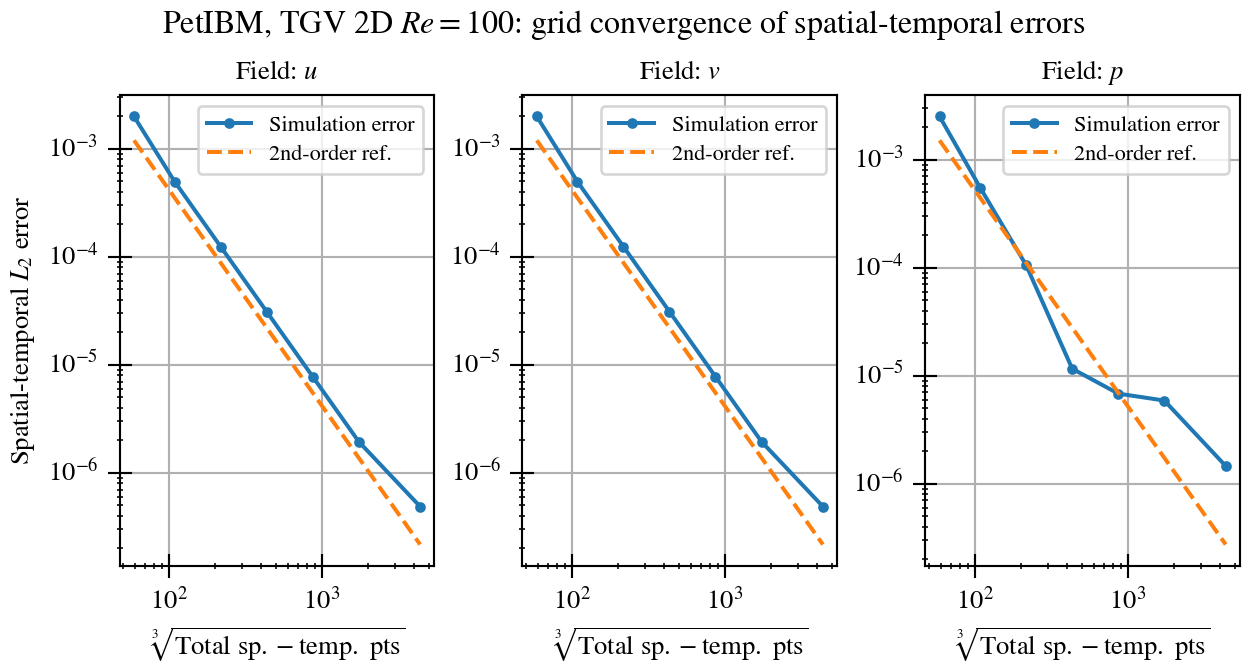
\includegraphics[width=\columnwidth]{tgv-2d-re100/petibm-tgv-2d-re100-convergence}%
    \caption{%
        Grid-convergence test of 2D TGV $Re=\num{100}$ w/ PetIBM
    }
    \label{fig:tgv-petibm-convergence}%
\end{figure}

\lipsum[1]

\begin{figure}[!hbt]
    \centering%
    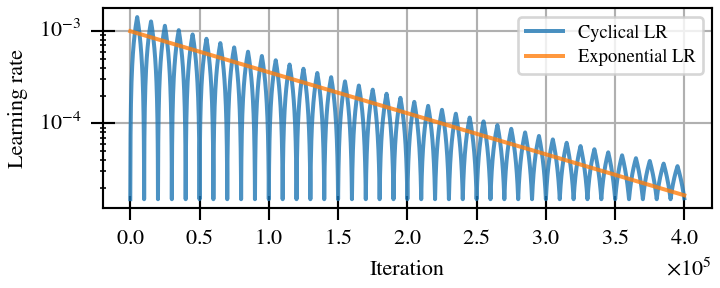
\includegraphics[width=\columnwidth]{tgv-2d-re100/learning-rate-hist}%
    \caption{%
        Learning-rate history of 2D TGV $Re=\num{100}$ w/ PINN
    }
    \label{fig:tgv-learning-rate-hist}%
\end{figure}

\lipsum[1]

\begin{figure}[!hbt]
    \centering%
    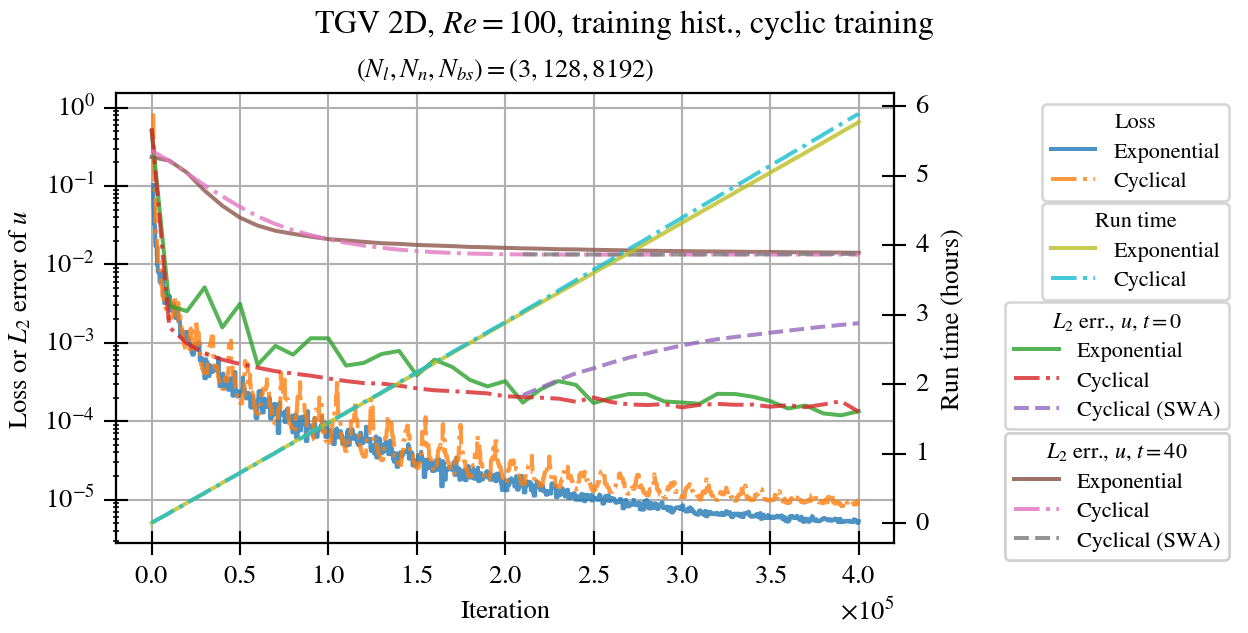
\includegraphics[width=\columnwidth]{tgv-2d-re100/pinn-nl3-nn128-npts8192-convergence}%
    \caption{%
        Training convergence history of 2D TGV $Re=\num{100}$ w/ PINN
    }
    \label{fig:tgv-pinn-loss}%
\end{figure}

\lipsum[1]

\begin{figure*}[!t]
    \centering%
    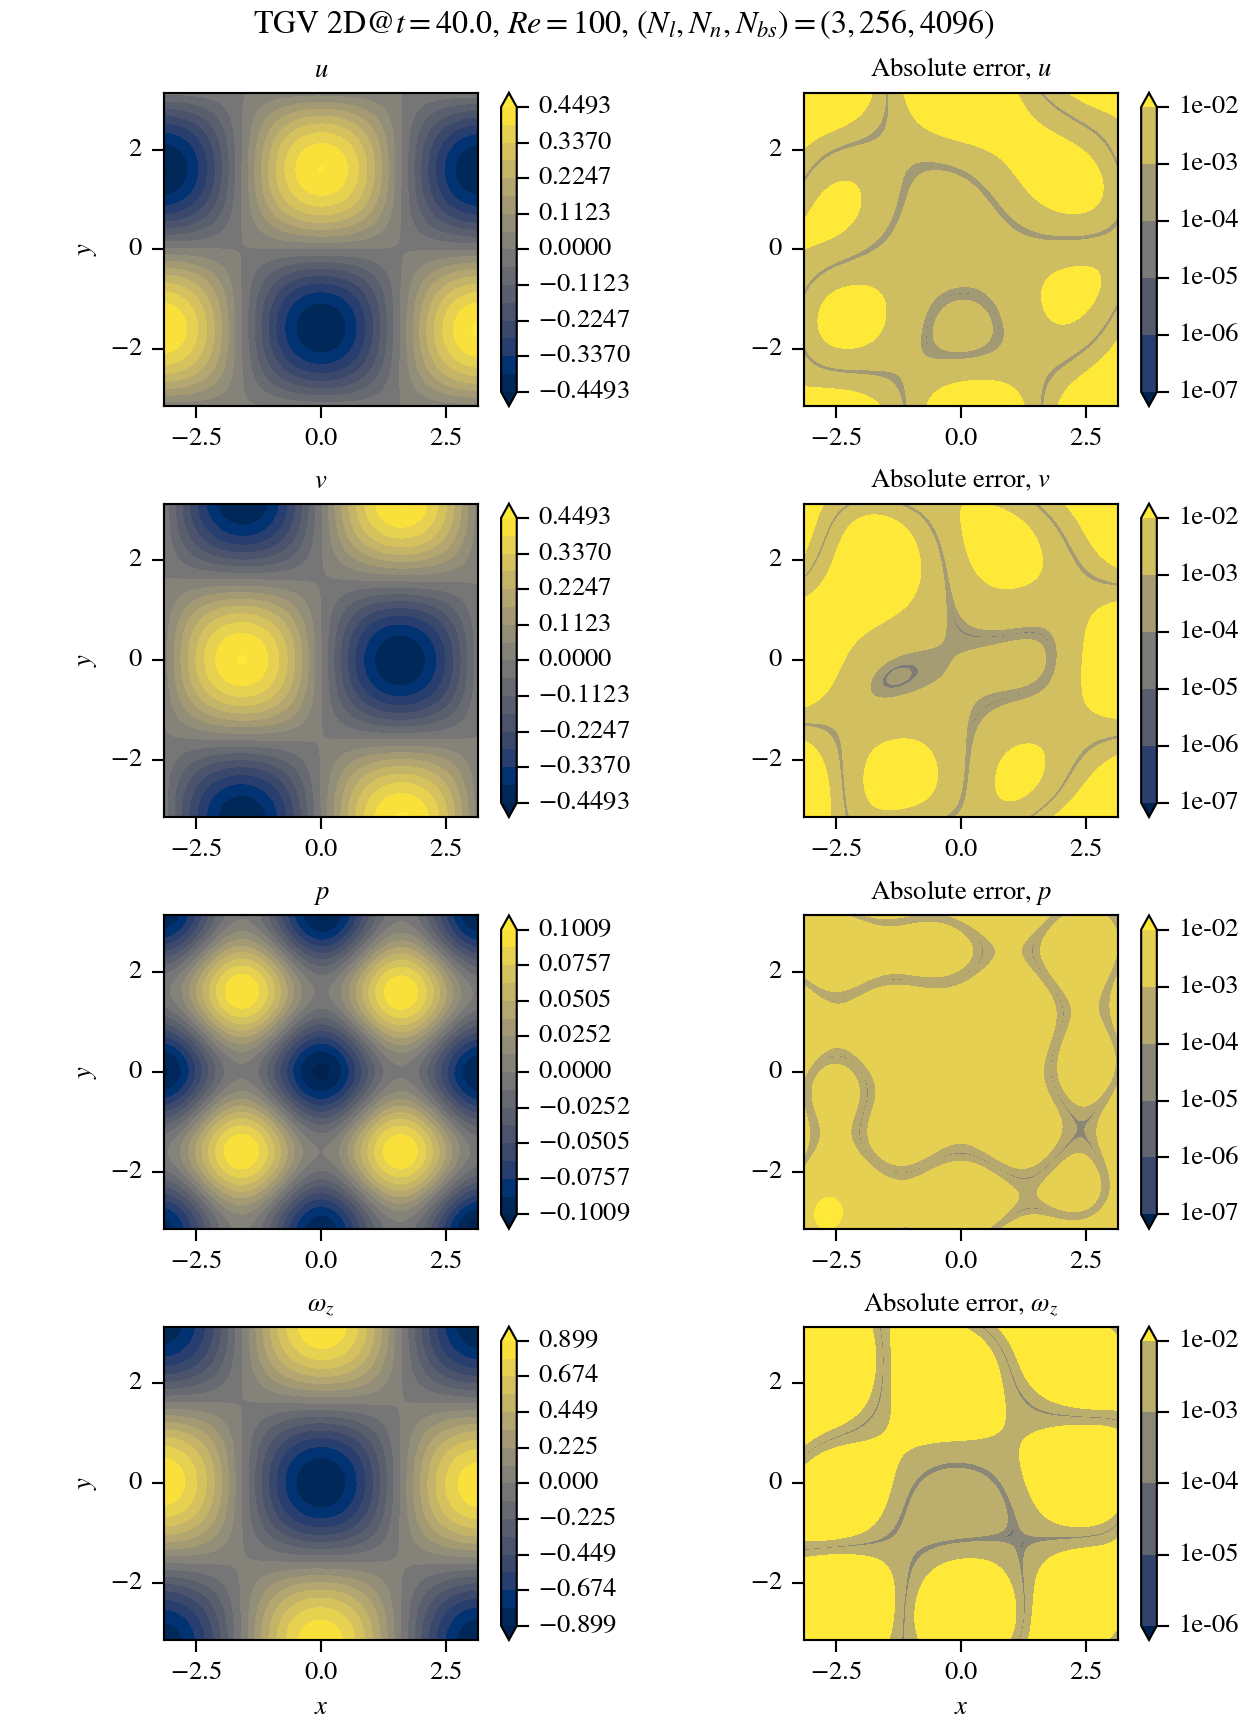
\includegraphics[width=0.8\linewidth]{tgv-2d-re100/pinn-nl3-nn256-npts4096-contours.png}%
    \caption{%
        Contours of 2D TGV $Re=\num{100}$ w/ PINN
    }
    \label{fig:tgv-pinn-contours}%
\end{figure*}

\lipsum[1]

\subsection{Verification and Validation: 2D Cylinder, $Re=\num{40}$}

\lipsum[1]

\begin{figure}[!hbt]
    \centering%
    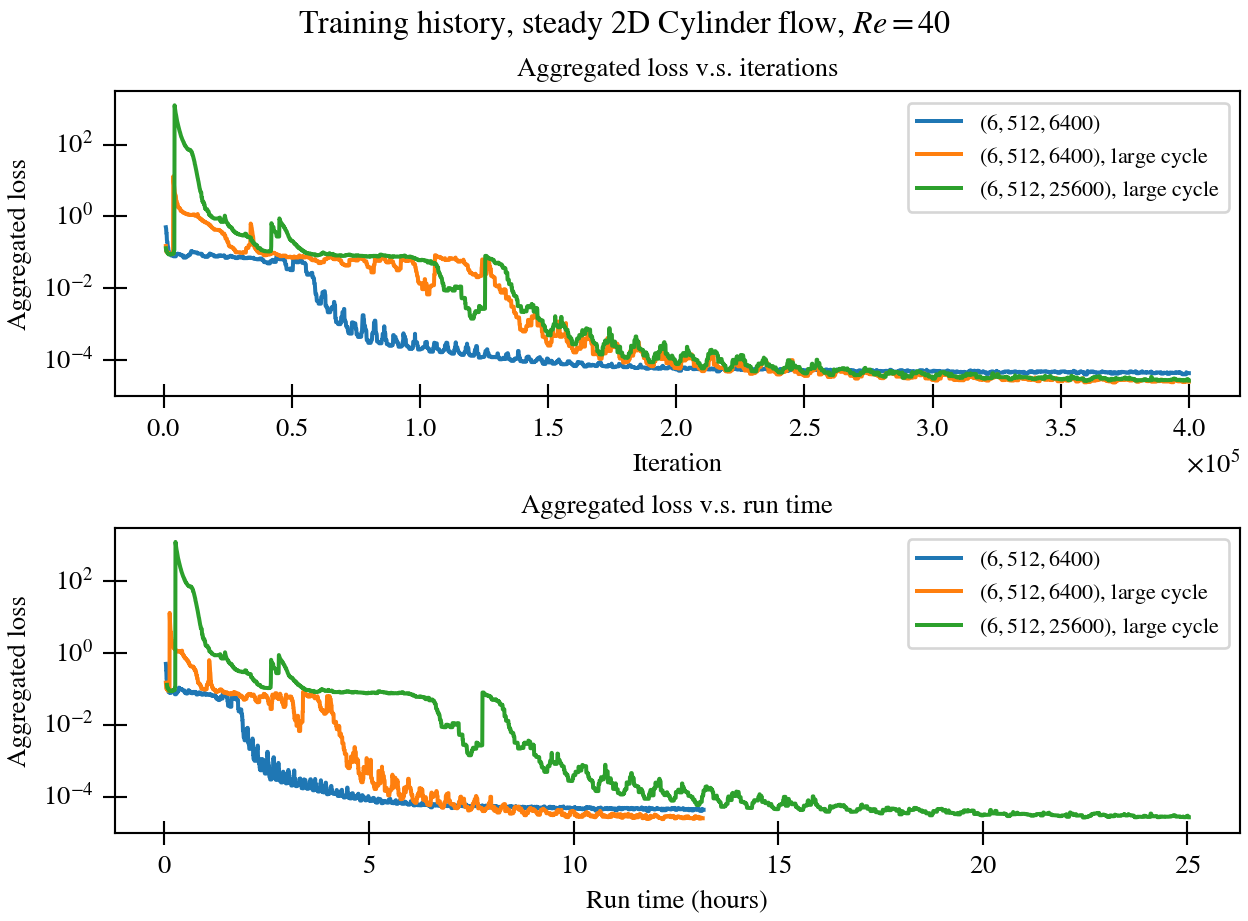
\includegraphics[width=0.95\columnwidth]{cylinder-2d-re40/loss-hist-steady.png}%
    \caption{%
        Training convergence history of 2D cylinder flow at $Re=\num{40}$ w/ steady PINN
    }
    \label{fig:cylinder-re40-steady-pinn-loss}%
\end{figure}

\lipsum[1]

\begin{figure}[!hbt]
    \centering%
    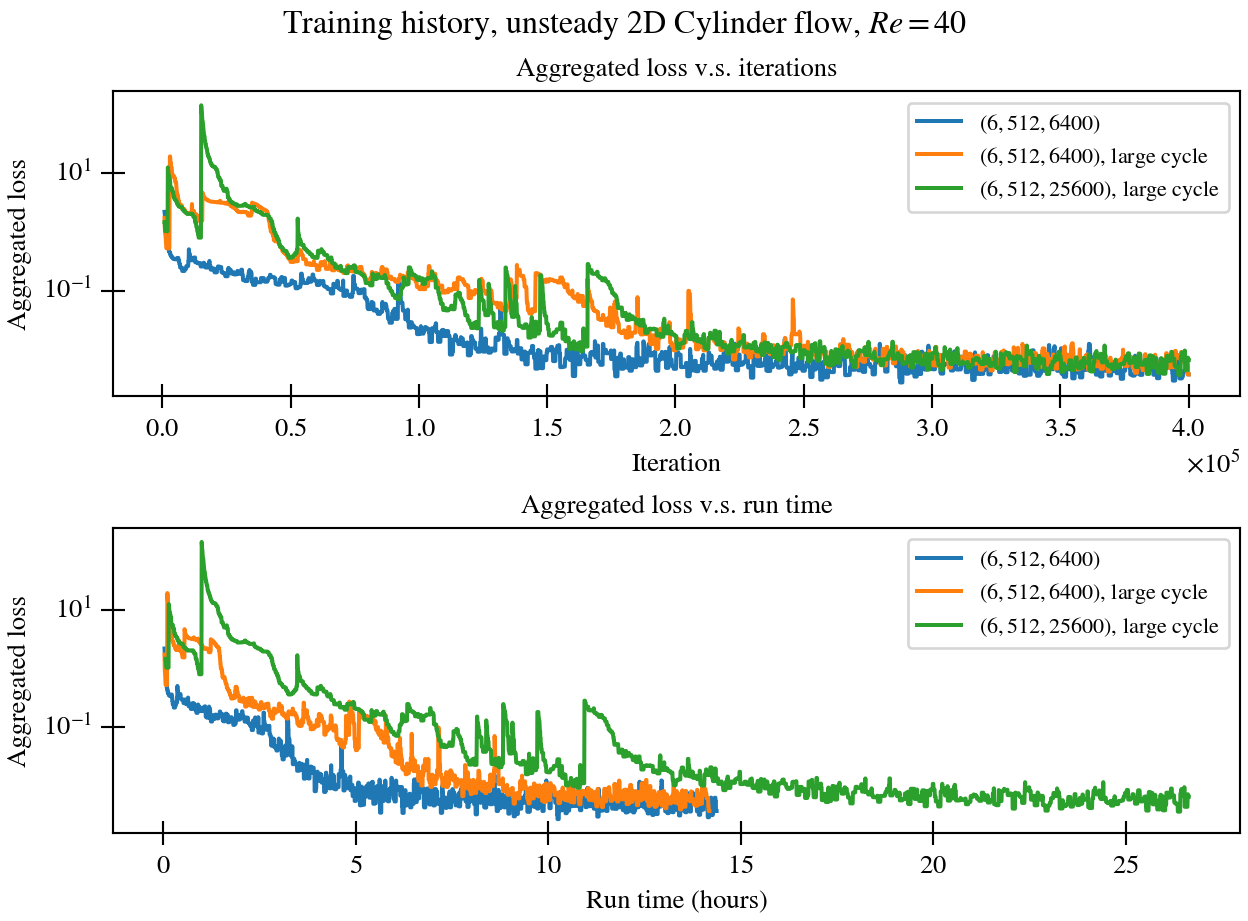
\includegraphics[width=0.95\columnwidth]{cylinder-2d-re40/loss-hist-unsteady.png}%
    \caption{%
        Training convergence history of 2D cylinder flow at $Re=\num{40}$ w/ unsteady PINN
    }
    \label{fig:cylinder-re40-unsteady-pinn-loss}%
\end{figure}

\lipsum[1]

\begin{table}[hbt!]
    \begin{threeparttable}[b]
        \begin{tabular}{lccc}
            \toprule
            & $C_D$ & $C_{D_p}$ & $C_{D_f}$ \\
            \midrule
            $(6, 512, 6400)$, steady & 1.62 & 1.07 & 0.55 \\
            $(6, 512, 6400)$, unsteady & 1.63 & 1.02 & 0.61 \\
            $(6, 512, 6400)$, large cycle, steady & 1.62 & 1.07 & 0.55 \\
            $(6, 512, 6400)$, large cycle, unsteady & 1.53 & 0.96 & 0.57 \\
            $(6, 512, 25600)$, large cycle, steady & 1.62 & 1.06 & 0.55 \\
            $(6, 512, 25600)$, large cycle, unsteady & 1.60 & 1.06 & 0.55 \\
            PetIBM & 1.63 & 1.02 & 0.61 \\
            Rosetti et al., 2012\cite{rosetti_urans_2012}\tnote{1} & \num{1.74+-0.09} & n/a & n/a \\
            Rosetti et al., 2012\cite{rosetti_urans_2012}\tnote{2} & 1.61 & n/a & n/a \\
            Sen et al., 2009\cite{sen_steady_2009}\tnote{2} & 1.51 & n/a & n/a \\
            Park et al., 1988\cite{park_numerical_1998}\tnote{2} & 1.51 & 0.99 & 0.53 \\
            Tritton, 1959\cite{tritton_experiments_1959}\tnote{1} & 1.48--1.65 & n/a & n/a \\
            Grove et al., 1964\cite{grove_experimental_1964}\tnote{1} & n/a & 0.94 & n/a \\
            \bottomrule
        \end{tabular}%
        \begin{tablenotes}
            \footnotesize
            \item [1] Experimental result
            \item [2] Simulation result
        \end{tablenotes}
        \caption{%
            Validation of drag coefficients.%
            $C_D$, $C_{D_p}$, and $C_{D_f}$ denote the coefficients of total drag, pressure drag, %
            and friction drag, respectively.%
        }%
        \label{table:cylinder-re40-cd-comparison}
    \end{threeparttable}
\end{table}%

\begin{figure}[!hbt]
    \centering%
    \includegraphics[width=0.95\columnwidth]{cylinder-2d-re40/drag-lift-coeffs}%
    \caption{%
        Drag and lift coefficients of 2D cylinder flow at $Re=\num{40}$ w/ PINNs
    }
    \label{fig:cylinder-re40-drag-lift}%
\end{figure}

\lipsum[1]

\begin{figure}[!hbt]
    \centering%
    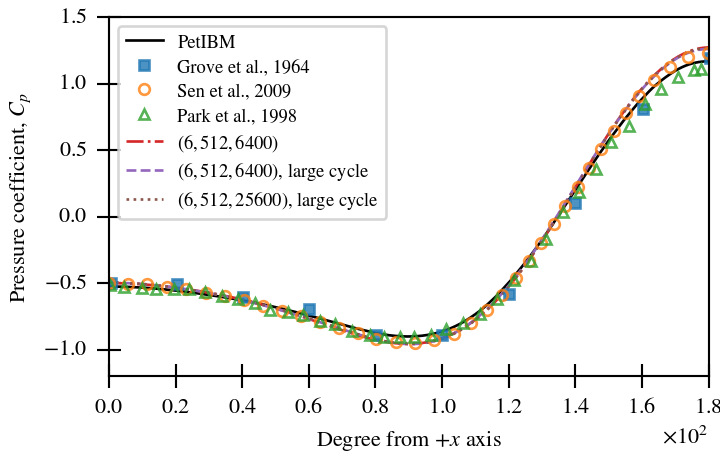
\includegraphics[width=0.95\columnwidth]{cylinder-2d-re40/surface-pressure-steady}%
    \caption{%
        Surface pressure distribution of 2D cylinder flow at $Re=\num{40}$ w/ steady PINN
    }
    \label{fig:cylinder-re40-steady-pinn-surfp}%
\end{figure}

\lipsum[1]

\begin{figure}[!hbt]
    \centering%
    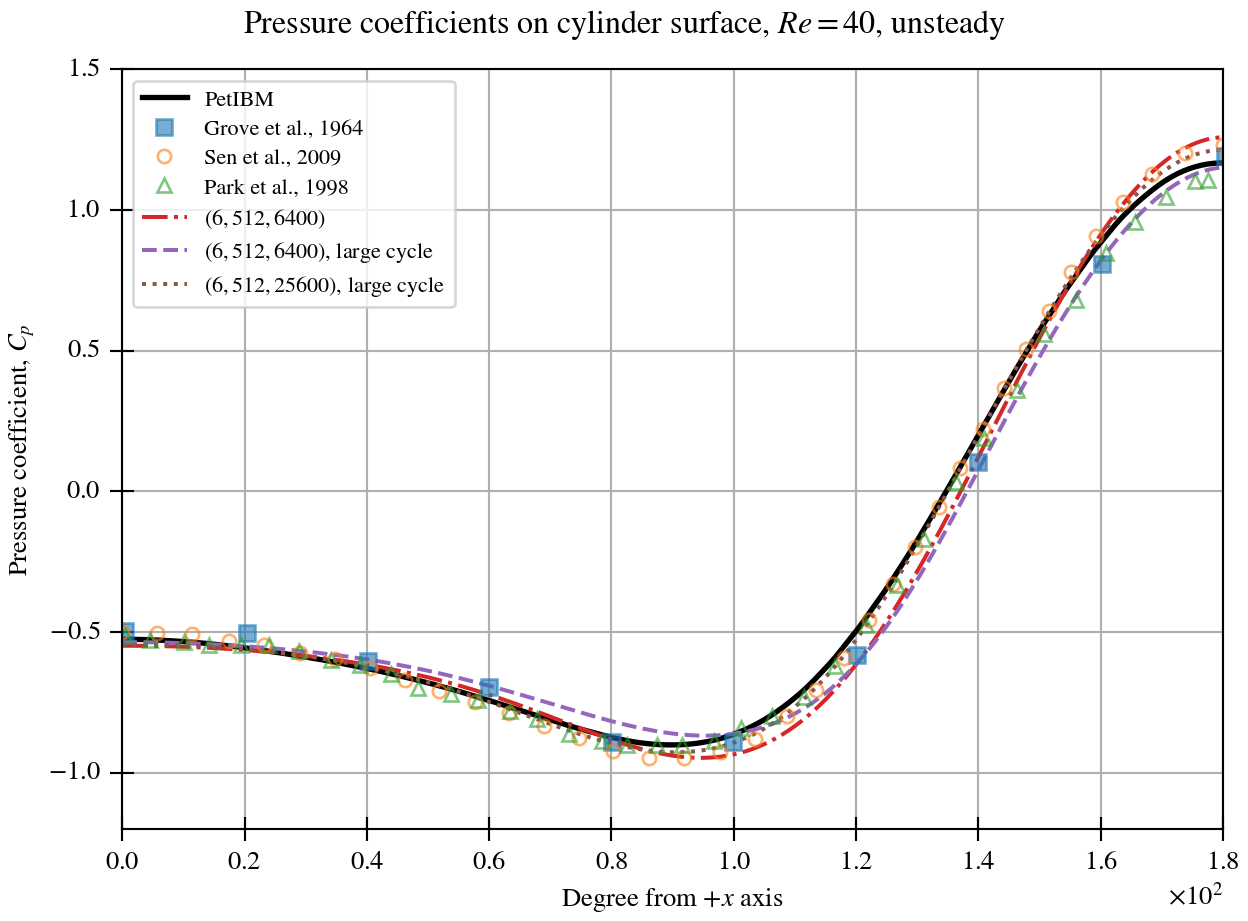
\includegraphics[width=0.95\columnwidth]{cylinder-2d-re40/surface-pressure-unsteady}%
    \caption{%
        Surface pressure distribution of 2D cylinder flow at $Re=\num{40}$ w/ unsteady PINN
    }
    \label{fig:cylinder-re40-unsteady-pinn-surfp}%
\end{figure}

\lipsum[1]

\begin{figure*}[!t]
    \centering%
    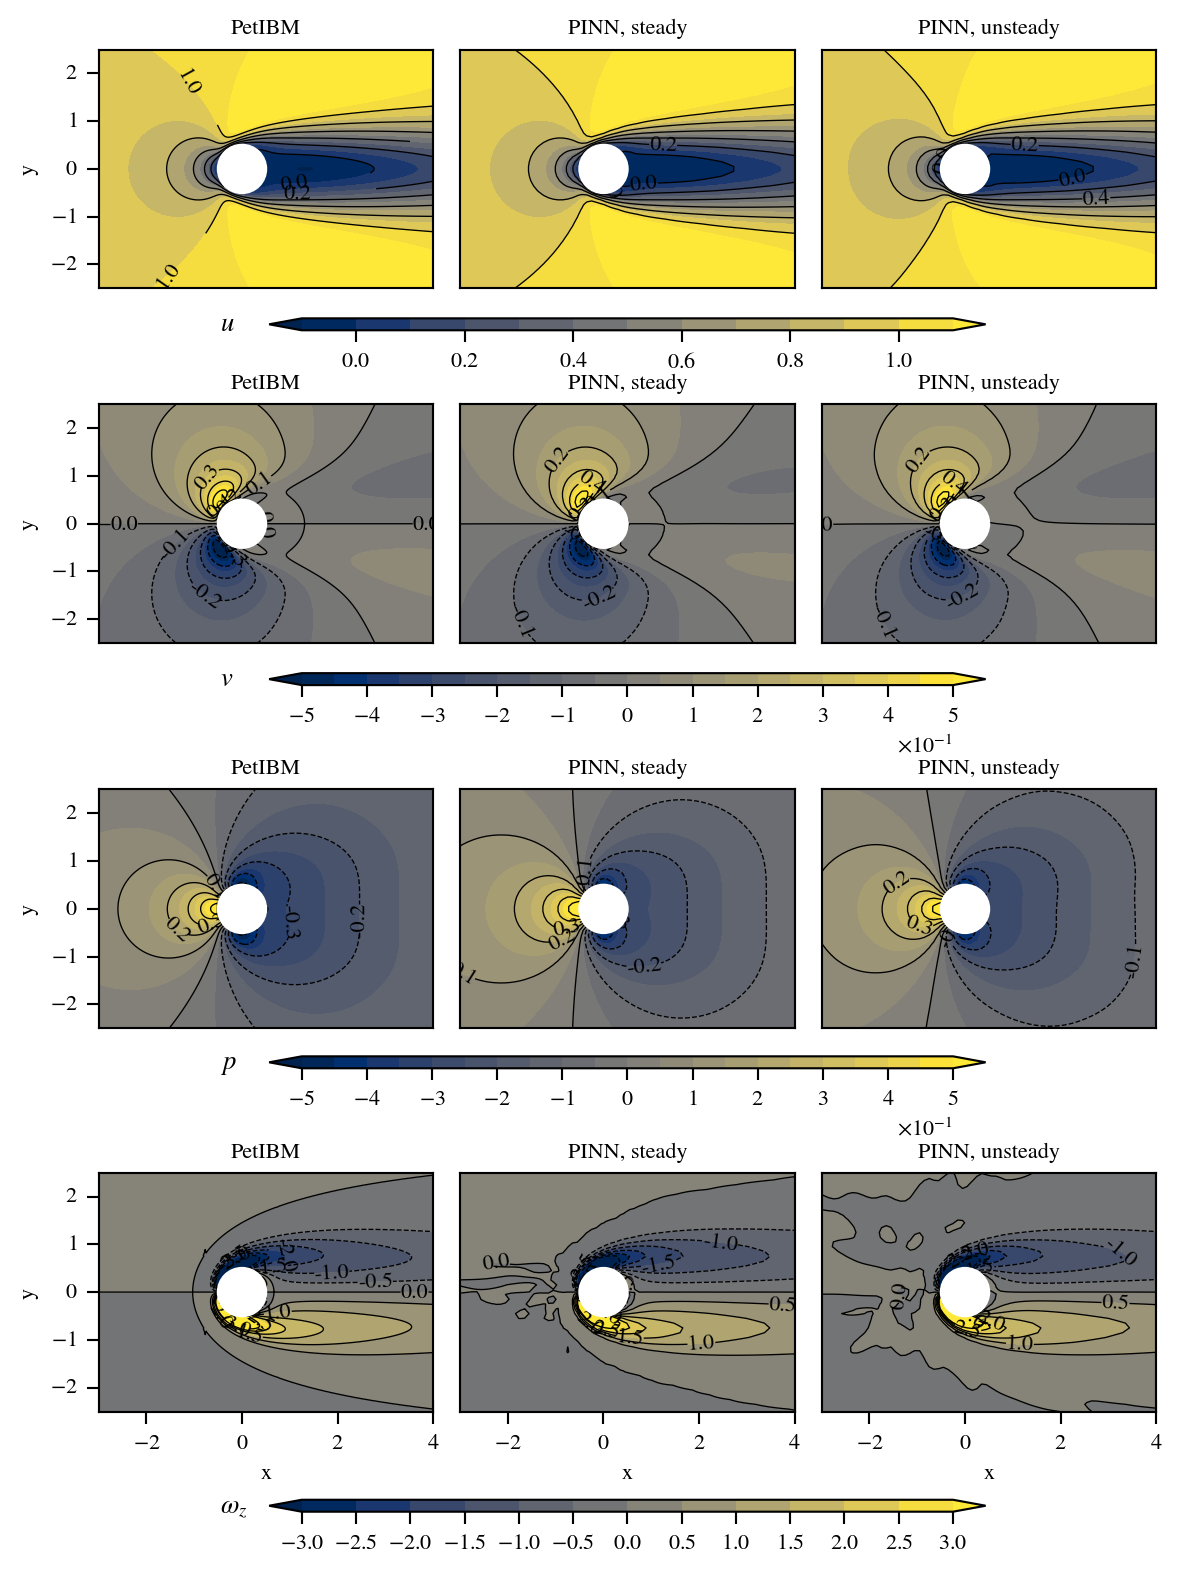
\includegraphics[width=0.85\linewidth]{cylinder-2d-re40/contour-comparison}%
    \caption{%
        Contour comparison of 2D cylinder flow at $Re=\num{40}$ w/ unsteady PINN
    }
    \label{fig:cylinder-re40-contours}%
\end{figure*}

\lipsum[1]

\subsection{2D Cylinder, $Re=\num{200}$}

\lipsum[1]

\begin{figure}[!hbt]
    \centering%
    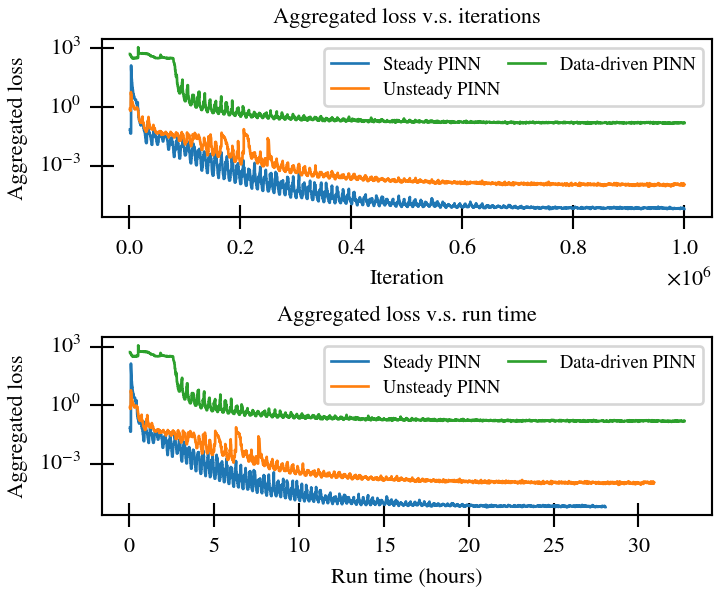
\includegraphics[width=0.95\columnwidth]{cylinder-2d-re200/loss-hist}%
    \caption{%
        Training convergence history of 2D cylinder flow at $Re=\num{200}$ w/ PINNs
    }
    \label{fig:cylinder-re200-pinn-loss}%
\end{figure}

\lipsum[1]

\begin{table}[hbt!]
    \begin{threeparttable}[b]
        \begin{tabular}{lcc}
            \toprule
            & $C_D$ \\
            \midrule
            PetIBM & 1.38   \\
            Steady PINN & 0.95 \\
            Unsteady PINN & 0.95 \\
            Deng et al., 2007\cite{deng_hydrodynamic_2007}\tnote{1} & 1.25 \\
            Rajani et al., 2009\cite{Rajani2009}\tnote{1} & 1.34 \\
            Gushchin \& Shchennikov, 1974\cite{gushchin_numerical_1974}\tnote{2} & 0.97 \\
            Fornberg, 1980\cite{fornberg_numerical_1980}\tnote{2} & 0.83 \\
            \bottomrule
        \end{tabular}%
        \begin{tablenotes}
            \footnotesize
            \item [1] Unsteady simulations.
            \item [2] Steady simulations.
        \end{tablenotes}
        \caption{%
            PINNs, 2D Cylinder, $Re=200$: validation of drag coefficients.%
            The data-driven case is excluded because it does not have an obvious periodic state nor a steady-state solution.%
        }%
        \label{table:cylinder-2d-re200-cd}
    \end{threeparttable}
\end{table}%

\begin{figure}[!hbt]
    \centering%
    \includegraphics[width=0.95\columnwidth]{cylinder-2d-re200/drag-lift-coeffs}%
    \caption{%
        Drag and lift coefficients of 2D cylinder flow at $Re=\num{200}$ w/ PINNs
    }
    \label{fig:cylinder-re200-drag-lift}%
\end{figure}

\lipsum[1]

\begin{figure}[!hbt]
    \centering%
    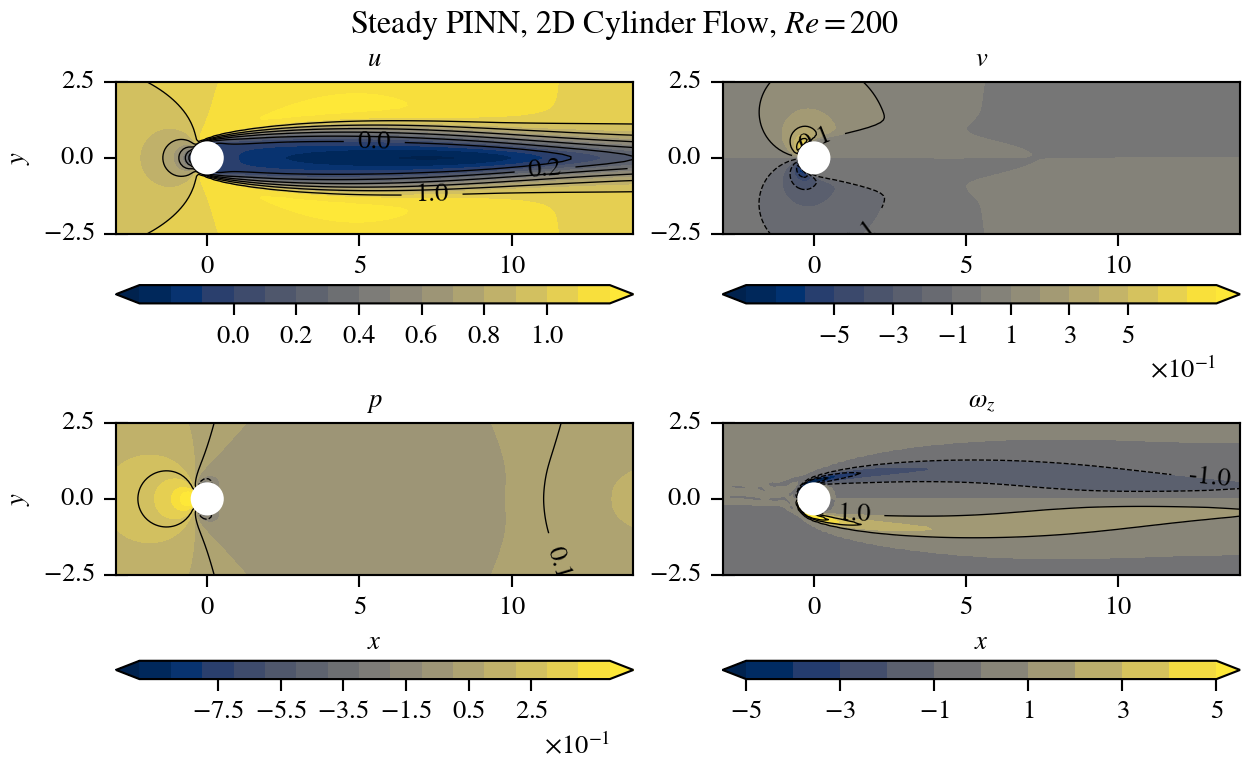
\includegraphics[width=0.95\columnwidth]{cylinder-2d-re200/contour-comparison-steady}%
    \caption{%
        Contours of 2D cylinder flow at $Re=\num{200}$ w/ steady PINN
    }
    \label{fig:cylinder-re200-steady-pinn-contours}%
\end{figure}

\begin{figure}[!hbt]
    \centering%
    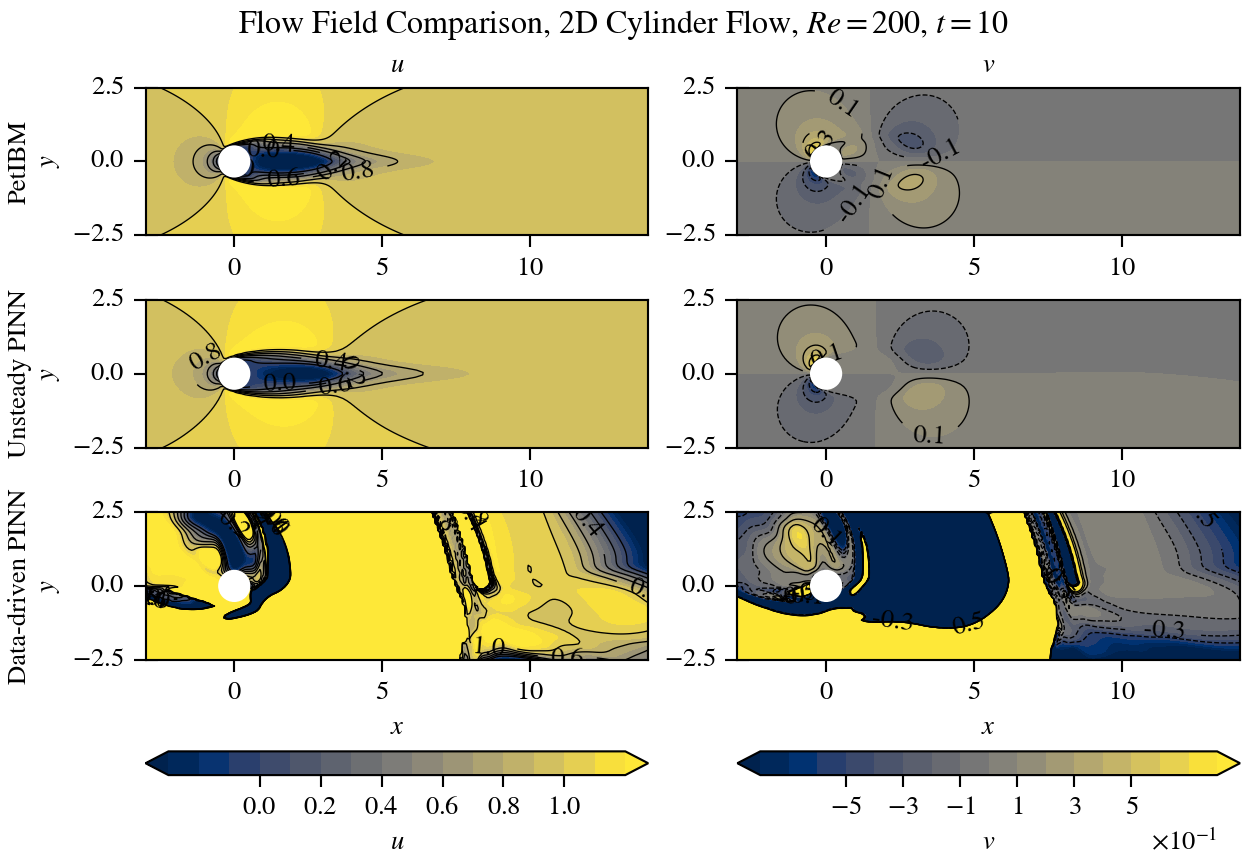
\includegraphics[width=0.95\columnwidth]{cylinder-2d-re200/contour-comparison-uv-t10}%
    \caption{%
        Contour comparison of 2D cylinder flow at $Re=\num{200}$ at $t=10$ w/ PINNs ($u$ and $v$ velocity)
    }
    \label{fig:cylinder-re200-pinn-contours-uv-t10}%
\end{figure}

\begin{figure}[!hbt]
    \centering%
    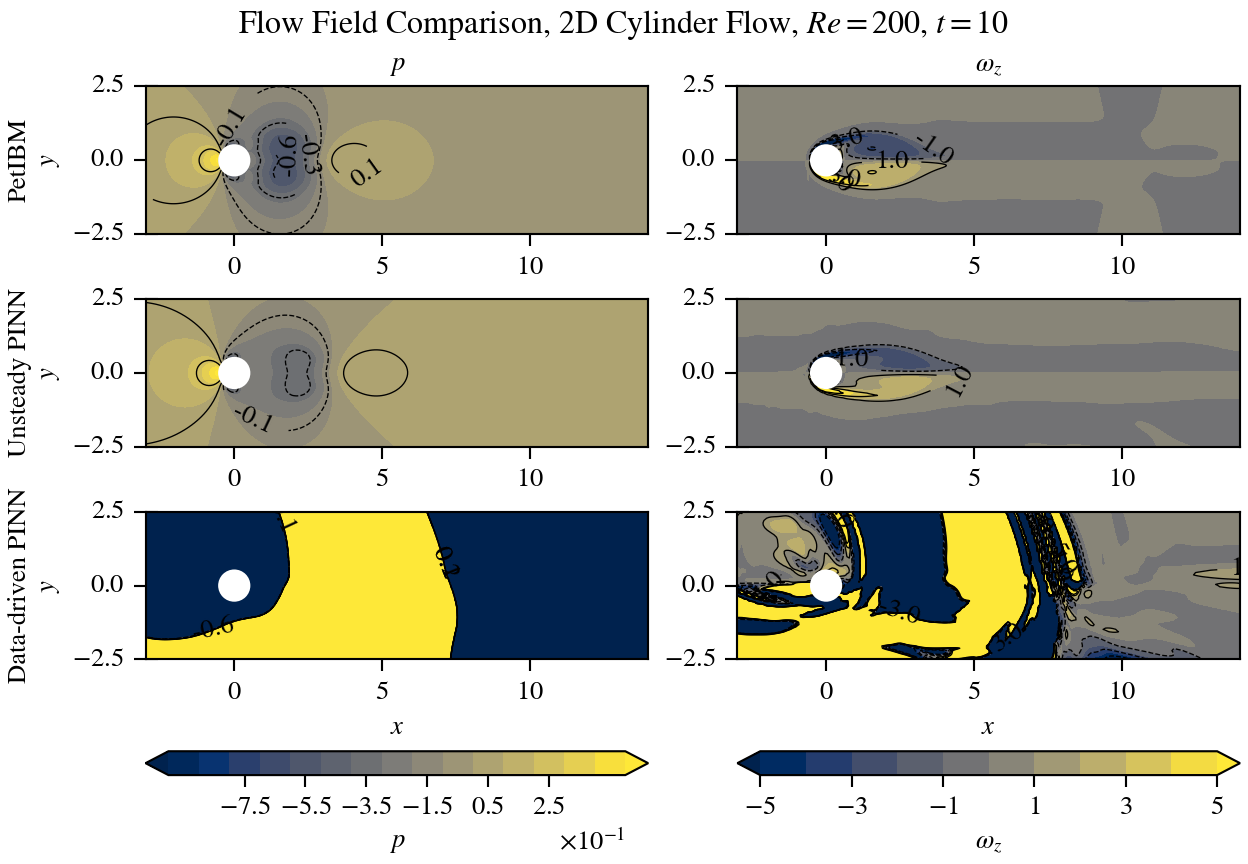
\includegraphics[width=0.95\columnwidth]{cylinder-2d-re200/contour-comparison-pwz-t10}%
    \caption{%
        Contour comparison of 2D cylinder flow at $Re=\num{200}$ at $t=10$ w/ PINNs (pressure and vorticity)
    }
    \label{fig:cylinder-re200-pinn-contours-pwz-t10}%
\end{figure}

\begin{figure}[!hbt]
    \centering%
    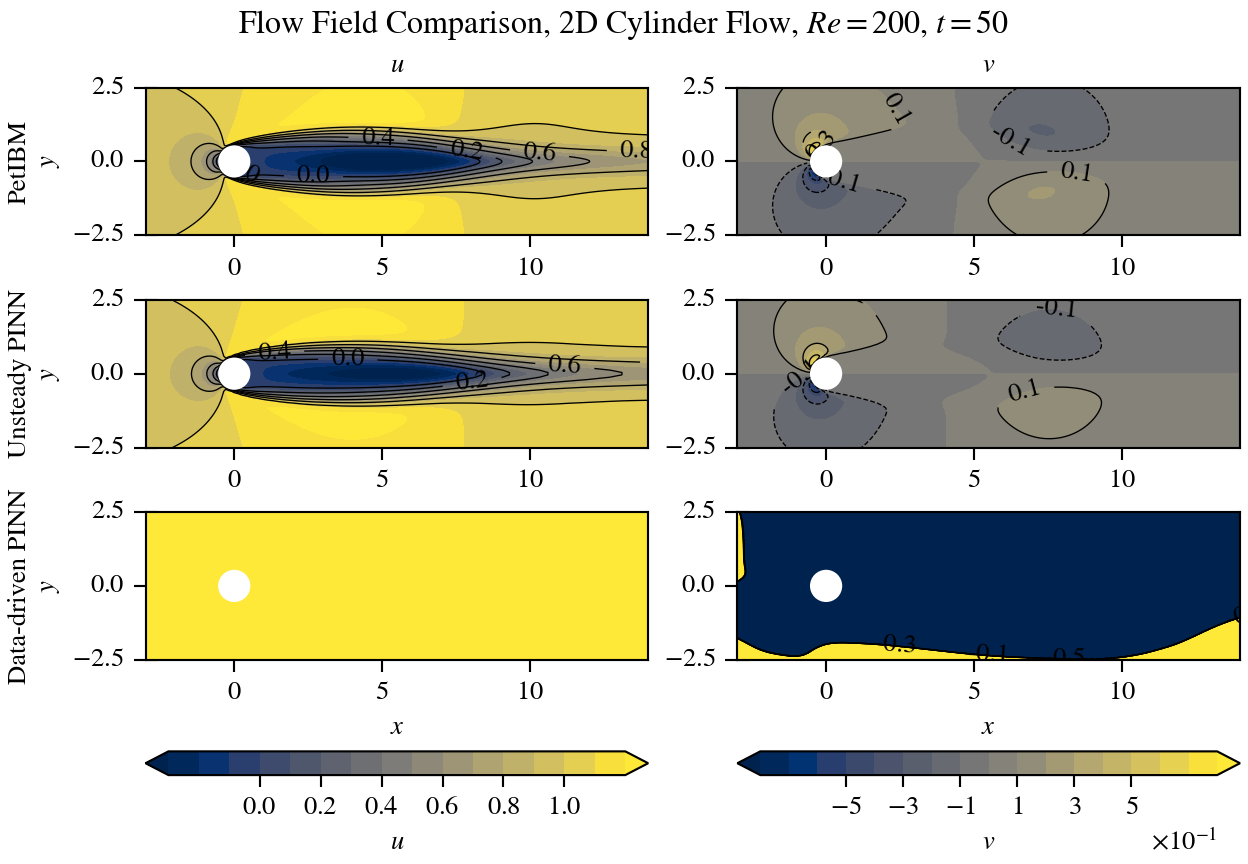
\includegraphics[width=0.95\columnwidth]{cylinder-2d-re200/contour-comparison-uv-t50}%
    \caption{%
        Contour comparison of 2D cylinder flow at $Re=\num{200}$ at $t=50$ w/ PINNs ($u$ and $v$ velocity)
    }
    \label{fig:cylinder-re200-pinn-contours-uv-t50}%
\end{figure}

\begin{figure}[!hbt]
    \centering%
    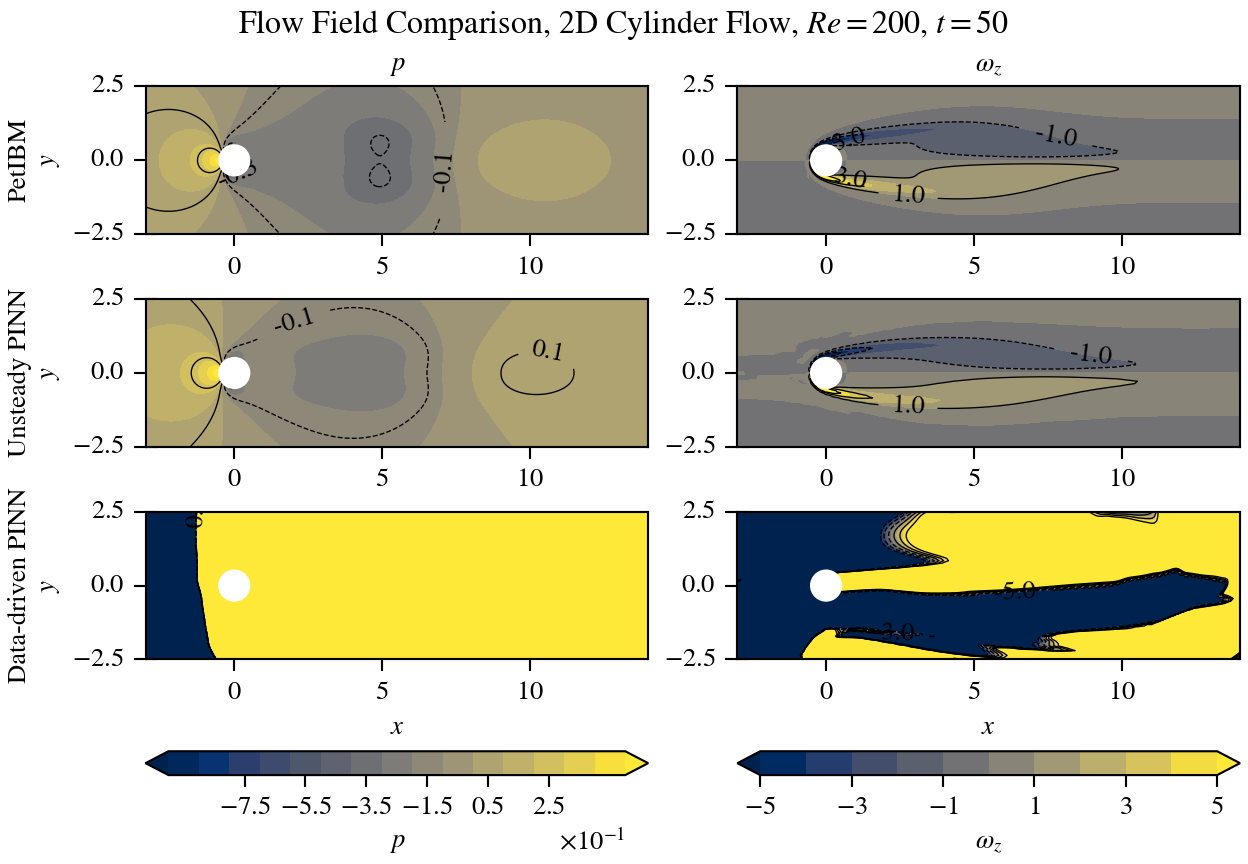
\includegraphics[width=0.95\columnwidth]{cylinder-2d-re200/contour-comparison-pwz-t50}%
    \caption{%
        Contour comparison of 2D cylinder flow at $Re=\num{200}$ at $t=50$ w/ PINNs (pressure and vorticity)
    }
    \label{fig:cylinder-re200-pinn-contours-pwz-t50}%
\end{figure}

\begin{figure}[!hbt]
    \centering%
    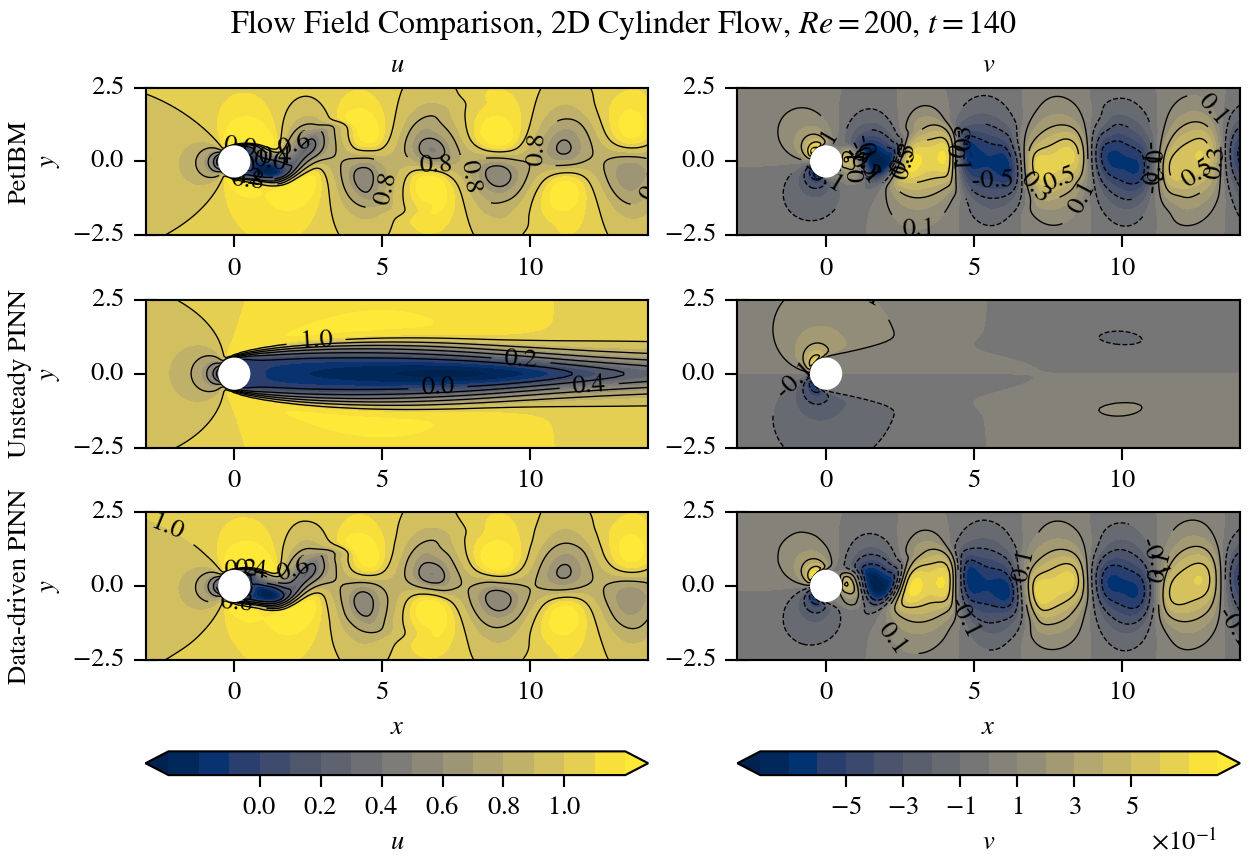
\includegraphics[width=0.95\columnwidth]{cylinder-2d-re200/contour-comparison-uv-t140}%
    \caption{%
        Contour comparison of 2D cylinder flow at $Re=\num{200}$ at $t=140$ w/ PINNs ($u$ and $v$ velocity)
    }
    \label{fig:cylinder-re200-pinn-contours-uv-t140}%
\end{figure}

\begin{figure}[!hbt]
    \centering%
    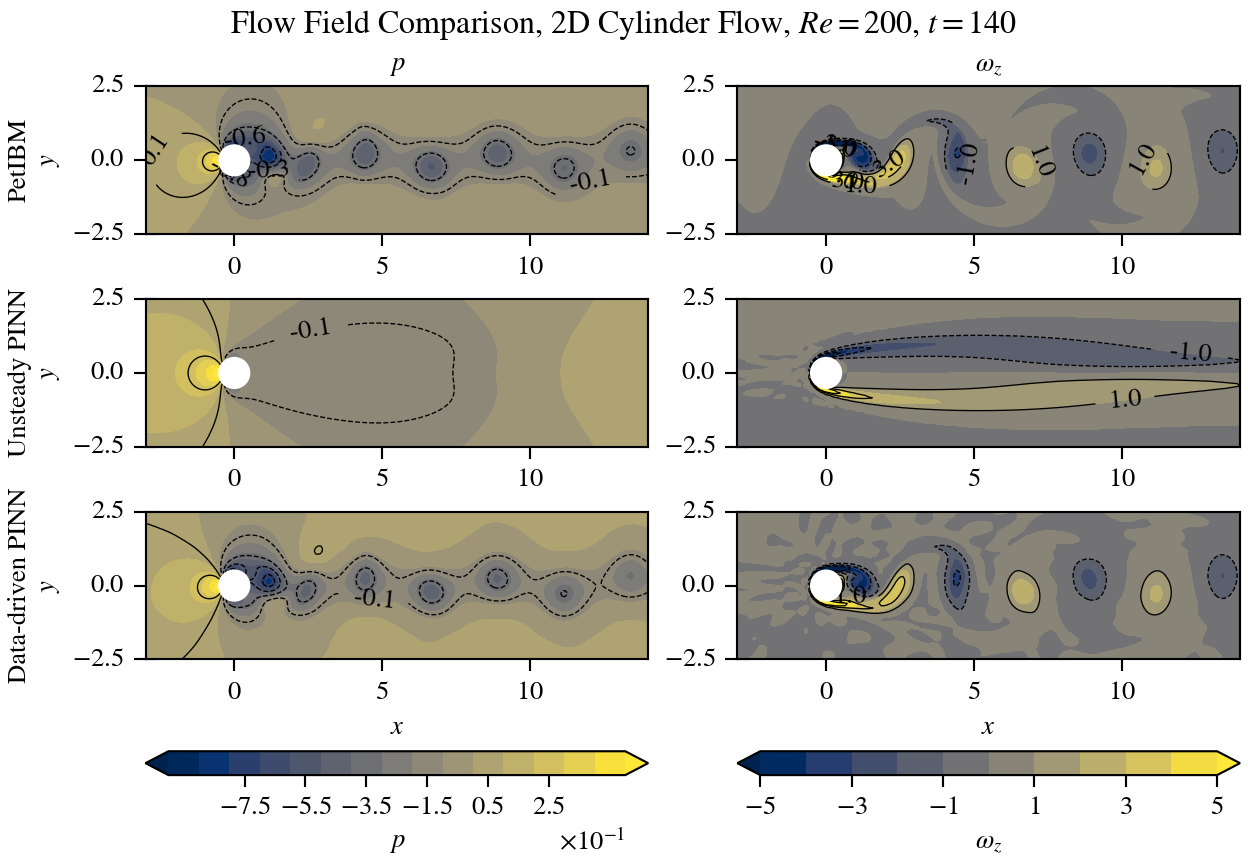
\includegraphics[width=0.95\columnwidth]{cylinder-2d-re200/contour-comparison-pwz-t140}%
    \caption{%
        Contour comparison of 2D cylinder flow at $Re=\num{200}$ at $t=140$ w/ PINNs (pressure and vorticity)
    }
    \label{fig:cylinder-re200-pinn-contours-pwz-t140}%
\end{figure}

\begin{figure}[!hbt]
    \centering%
    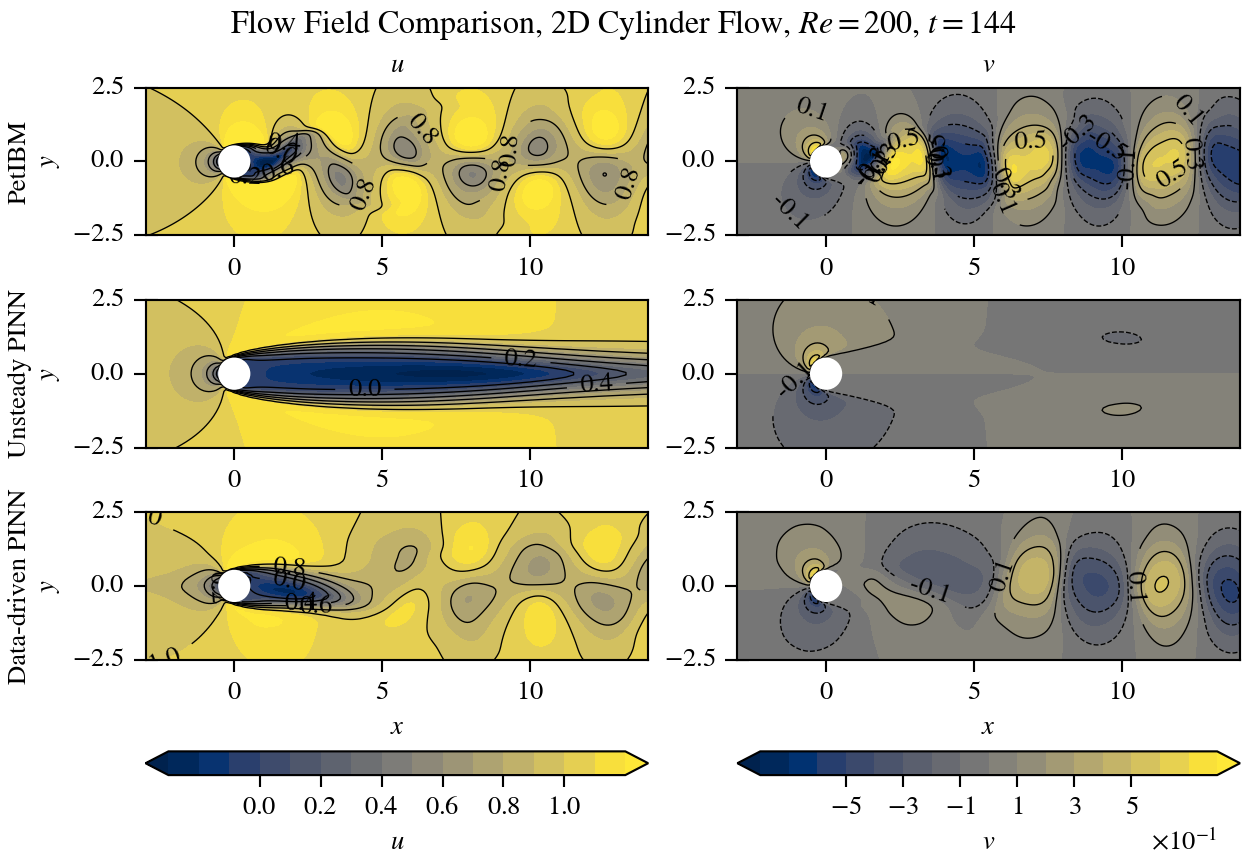
\includegraphics[width=0.95\columnwidth]{cylinder-2d-re200/contour-comparison-uv-t144}%
    \caption{%
        Contour comparison of 2D cylinder flow at $Re=\num{200}$ at $t=144$ w/ PINNs ($u$ and $v$ velocity)
    }
    \label{fig:cylinder-re200-pinn-contours-uv-t144}%
\end{figure}

\begin{figure}[!hbt]
    \centering%
    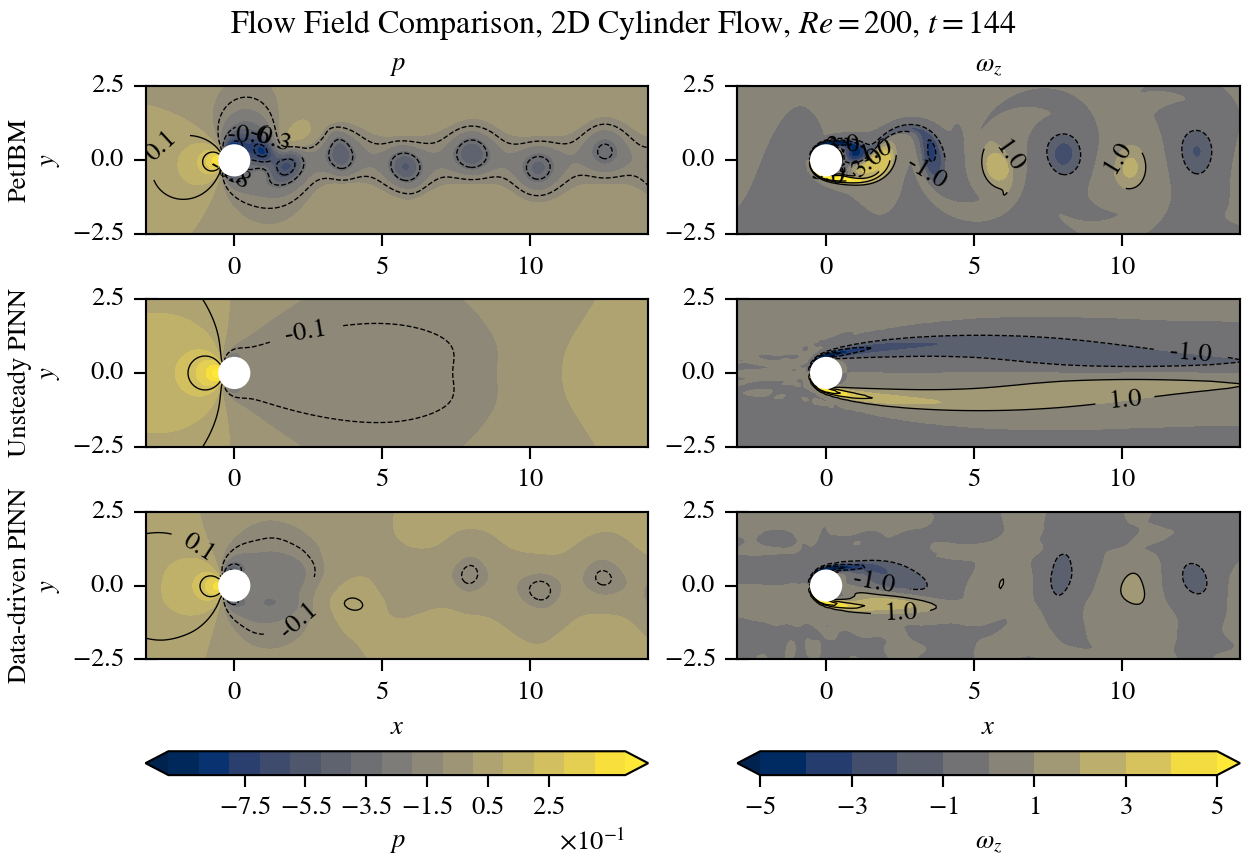
\includegraphics[width=0.95\columnwidth]{cylinder-2d-re200/contour-comparison-pwz-t144}%
    \caption{%
        Contour comparison of 2D cylinder flow at $Re=\num{200}$ at $t=144$ w/ PINNs (pressure and vorticity)
    }
    \label{fig:cylinder-re200-pinn-contours-pwz-t144}%
\end{figure}

\begin{figure}[!hbt]
    \centering%
    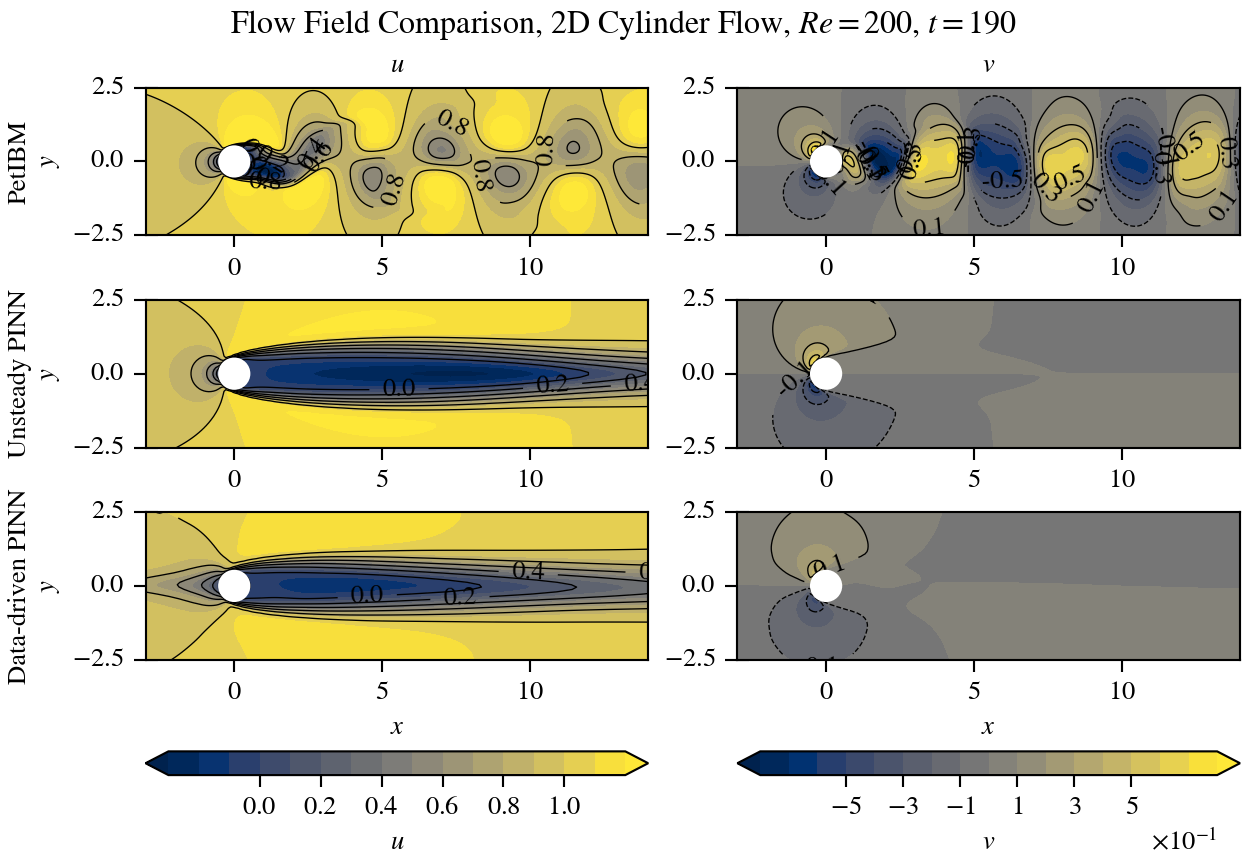
\includegraphics[width=0.95\columnwidth]{cylinder-2d-re200/contour-comparison-uv-t190}%
    \caption{%
        Contour comparison of 2D cylinder flow at $Re=\num{200}$ at $t=190$ w/ PINNs ($u$ and $v$ velocity)
    }
    \label{fig:cylinder-re200-pinn-contours-uv-t190}%
\end{figure}

\begin{figure}[!hbt]
    \centering%
    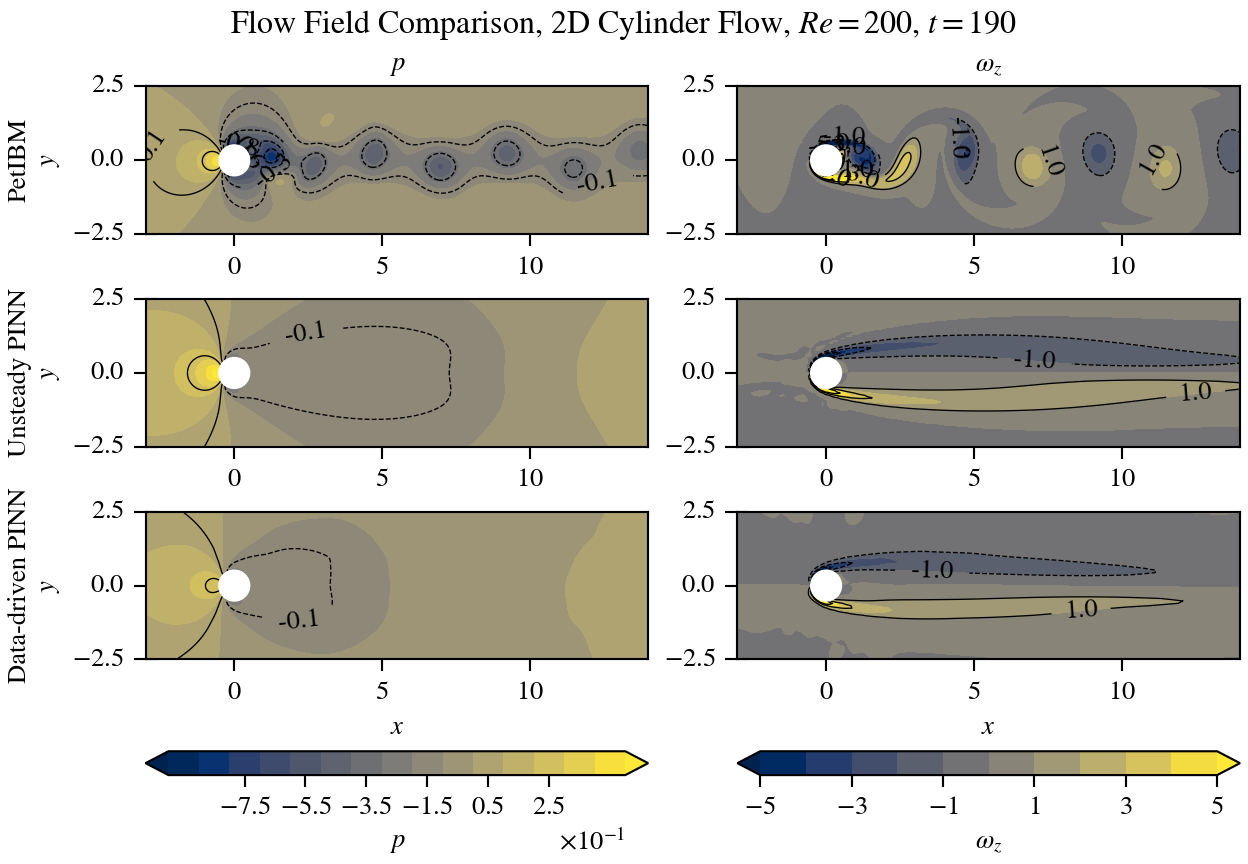
\includegraphics[width=0.95\columnwidth]{cylinder-2d-re200/contour-comparison-pwz-t190}%
    \caption{%
        Contour comparison of 2D cylinder flow at $Re=\num{200}$ at $t=190$ w/ PINNs (pressure and vorticity)
    }
    \label{fig:cylinder-re200-pinn-contours-pwz-t190}%
\end{figure}

\begin{figure}[!hbt]
    \centering%
    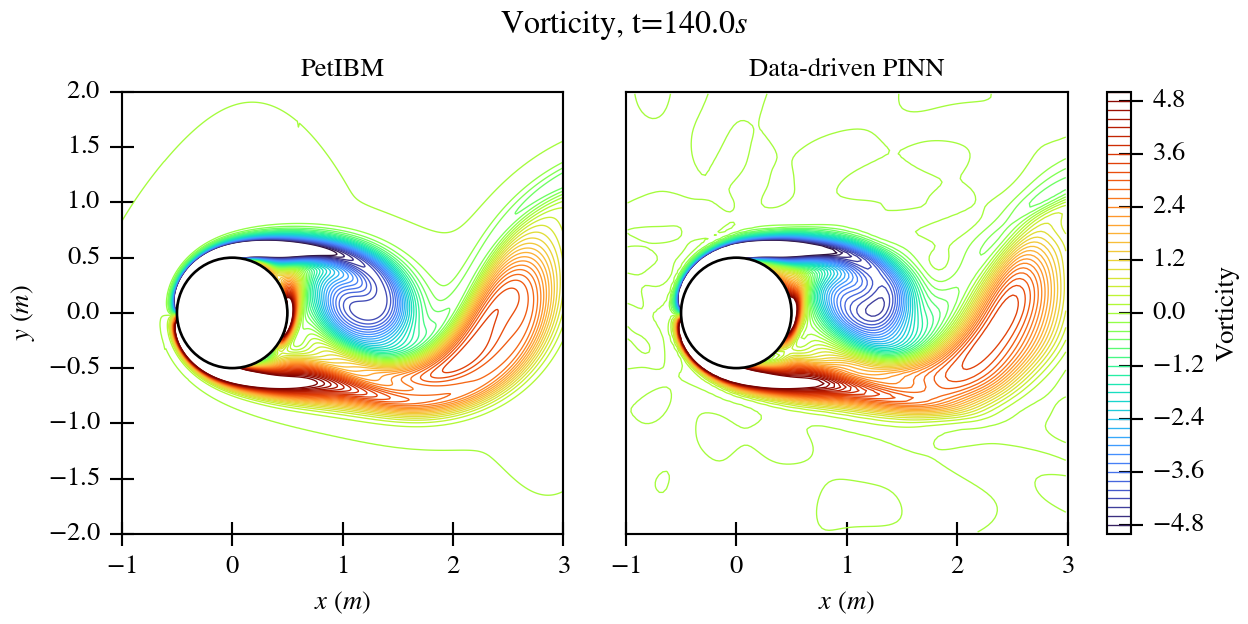
\includegraphics[width=0.95\columnwidth]{cylinder-2d-re200/vorticity_z_t140.0.png}%
    \caption{%
        Vorticity generation near the cylinder for 2D cylinder flow at $Re=\num{200}$ at $t=140$ w/ data-driven PINNs
    }
    \label{fig:cylinder-re200-pinn-vort-gen-t140.0}%
\end{figure}

\begin{figure}[!hbt]
    \centering%
    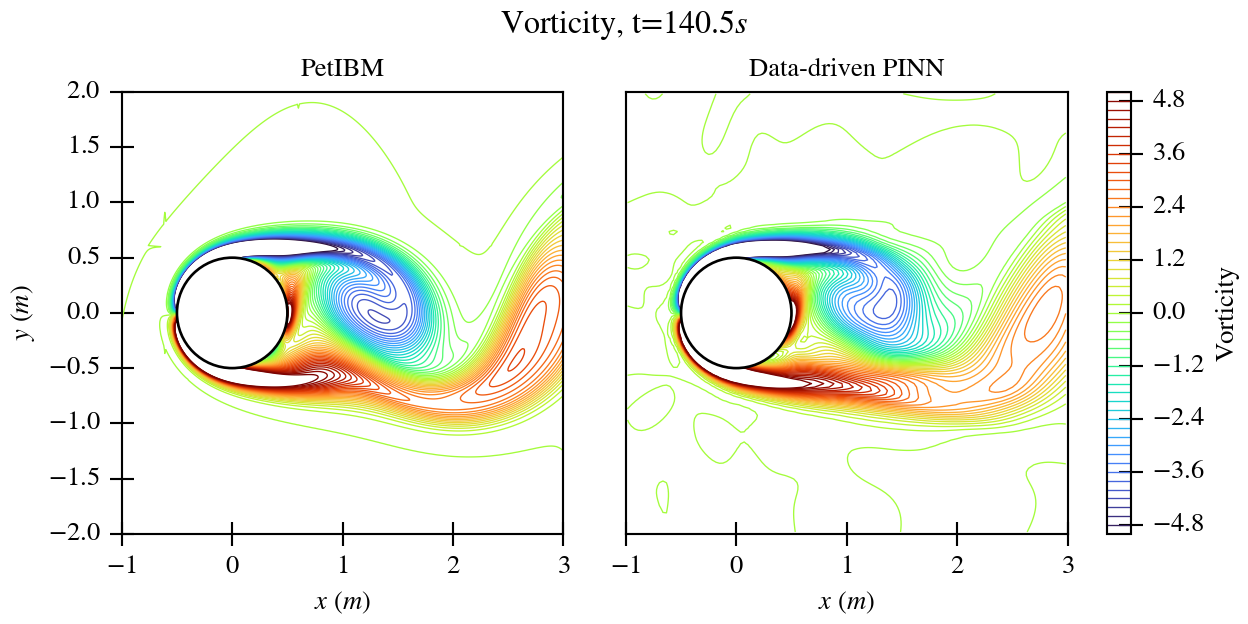
\includegraphics[width=0.95\columnwidth]{cylinder-2d-re200/vorticity_z_t140.5.png}%
    \caption{%
        Vorticity generation near the cylinder for 2D cylinder flow at $Re=\num{200}$ at $t=140.5$ w/ data-driven PINNs
    }
    \label{fig:cylinder-re200-pinn-vort-gen-t140.5}%
\end{figure}

\begin{figure}[!hbt]
    \centering%
    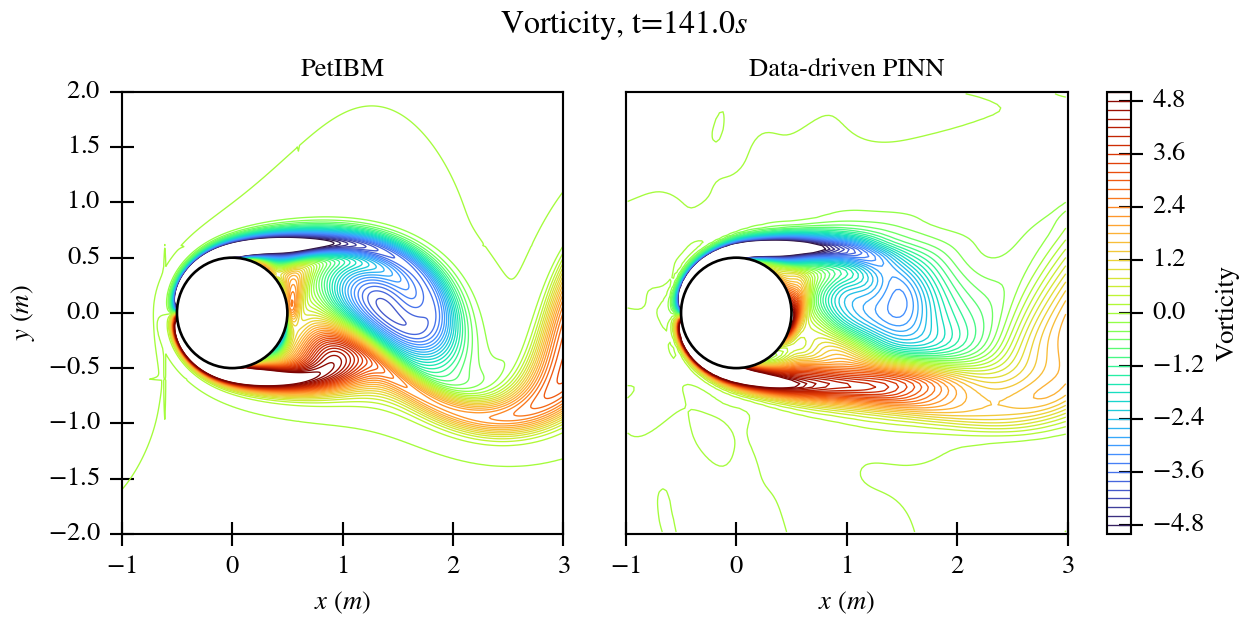
\includegraphics[width=0.95\columnwidth]{cylinder-2d-re200/vorticity_z_t141.0.png}%
    \caption{%
        Vorticity generation near the cylinder for 2D cylinder flow at $Re=\num{200}$ at $t=141$ w/ data-driven PINNs
    }
    \label{fig:cylinder-re200-pinn-vort-gen-t141.0}%
\end{figure}

\begin{figure}[!hbt]
    \centering%
    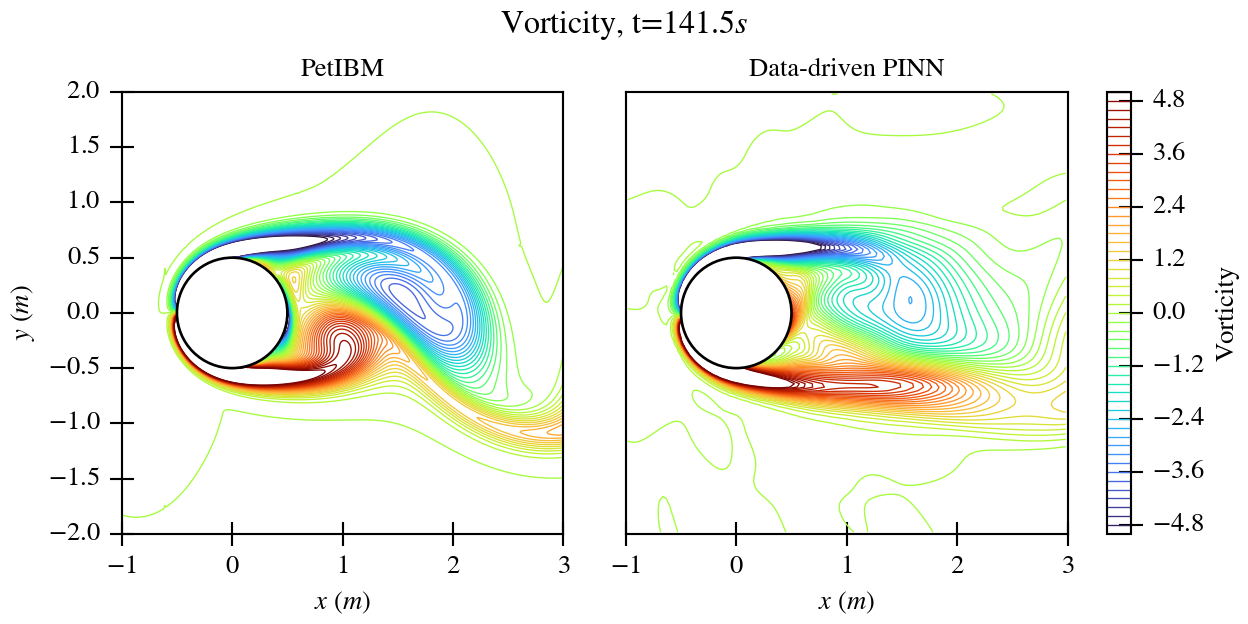
\includegraphics[width=0.95\columnwidth]{cylinder-2d-re200/vorticity_z_t141.5.png}%
    \caption{%
        Vorticity generation near the cylinder for 2D cylinder flow at $Re=\num{200}$ at $t=141.5$ w/ data-driven PINNs
    }
    \label{fig:cylinder-re200-pinn-vort-gen-t141.5}%
\end{figure}

\begin{figure}[!hbt]
    \centering%
    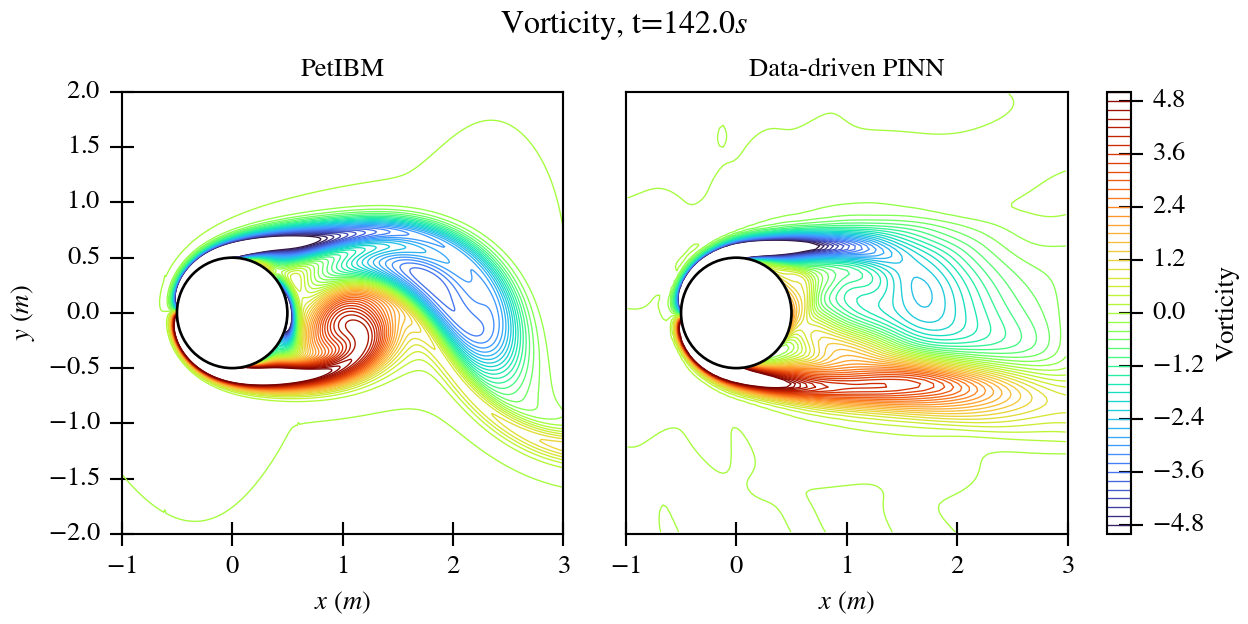
\includegraphics[width=0.95\columnwidth]{cylinder-2d-re200/vorticity_z_t142.0.png}%
    \caption{%
        Vorticity generation near the cylinder for 2D cylinder flow at $Re=\num{200}$ at $t=142$ w/ data-driven PINNs
    }
    \label{fig:cylinder-re200-pinn-vort-gen-t142.0}%
\end{figure}

\begin{figure}[!hbt]
    \centering%
    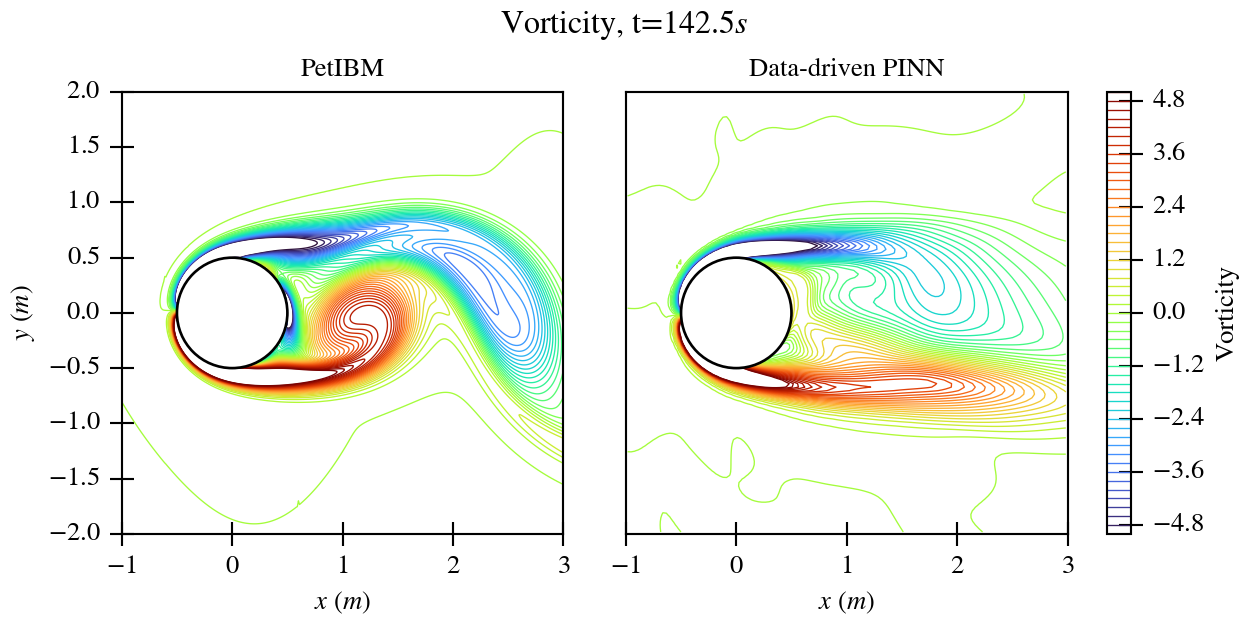
\includegraphics[width=0.95\columnwidth]{cylinder-2d-re200/vorticity_z_t142.5.png}%
    \caption{%
        Vorticity generation near the cylinder for 2D cylinder flow at $Re=\num{200}$ at $t=142.5$ w/ data-driven PINNs
    }
    \label{fig:cylinder-re200-pinn-vort-gen-t142.5}%
\end{figure}

\begin{figure}[!hbt]
    \centering%
    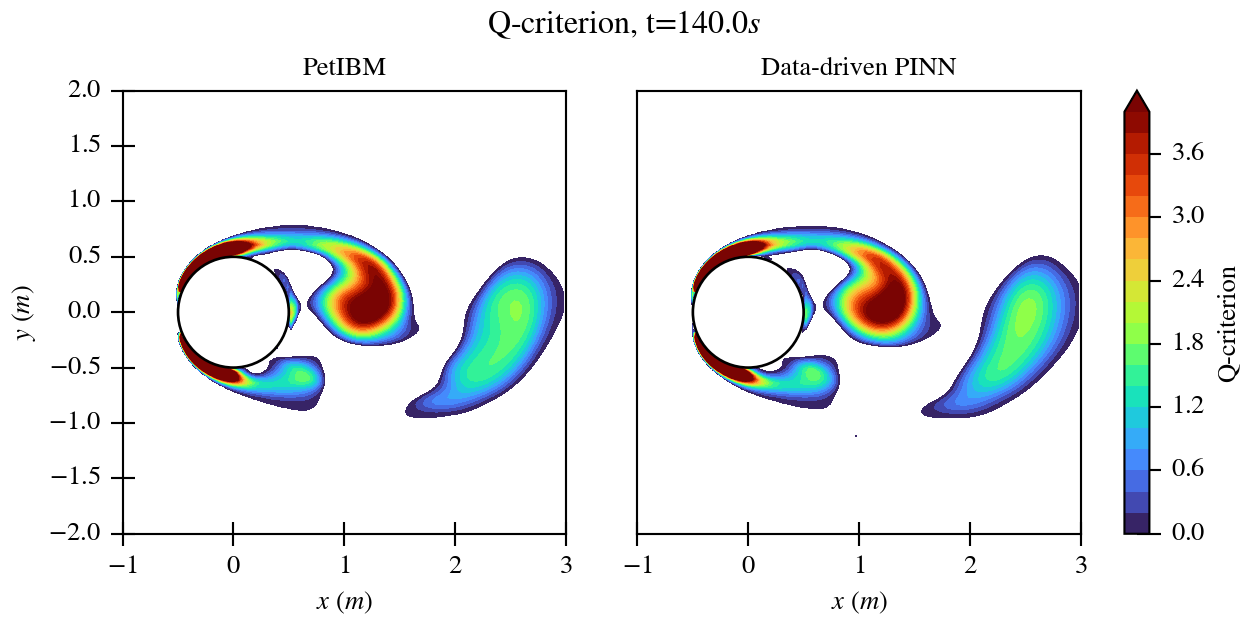
\includegraphics[width=0.95\columnwidth]{cylinder-2d-re200/qcriterion_t140.0.png}%
    \caption{%
        Q-criterion near the cylinder for 2D cylinder flow at $Re=\num{200}$ at $t=140$ w/ data-driven PINNs
    }
    \label{fig:cylinder-re200-pinn-qcrit-t140.0}%
\end{figure}

\begin{figure}[!hbt]
    \centering%
    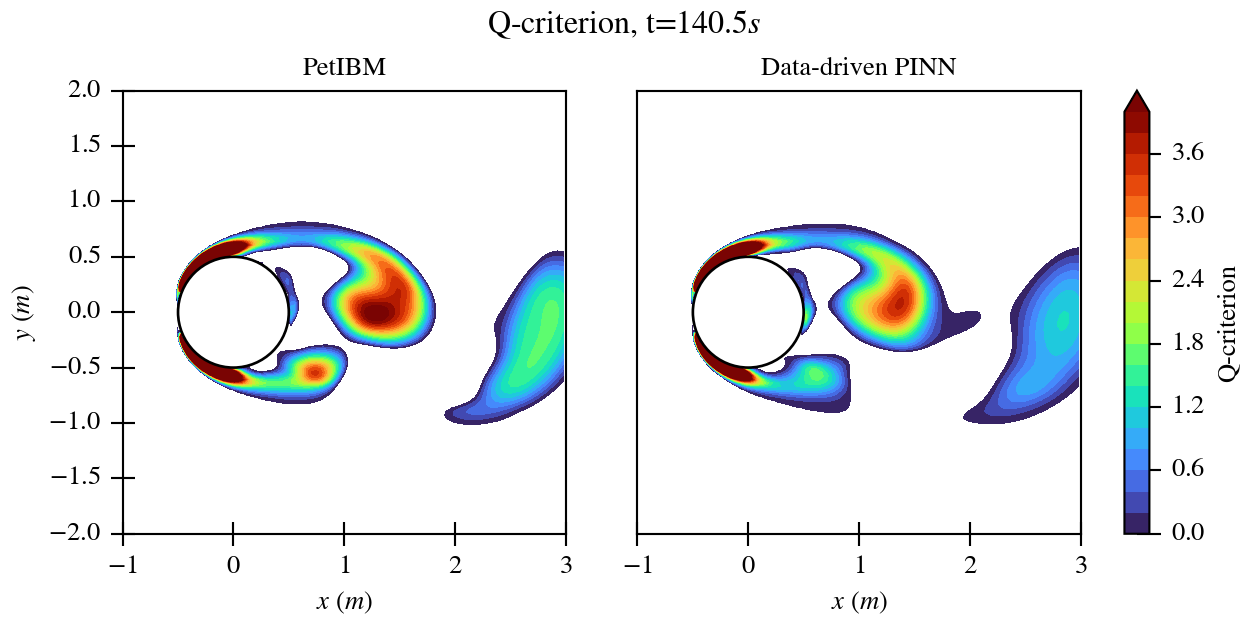
\includegraphics[width=0.95\columnwidth]{cylinder-2d-re200/qcriterion_t140.5.png}%
    \caption{%
        Q-criterion near the cylinder for 2D cylinder flow at $Re=\num{200}$ at $t=140.5$ w/ data-driven PINNs
    }
    \label{fig:cylinder-re200-pinn-qcrit-t140.5}%
\end{figure}

\begin{figure}[!hbt]
    \centering%
    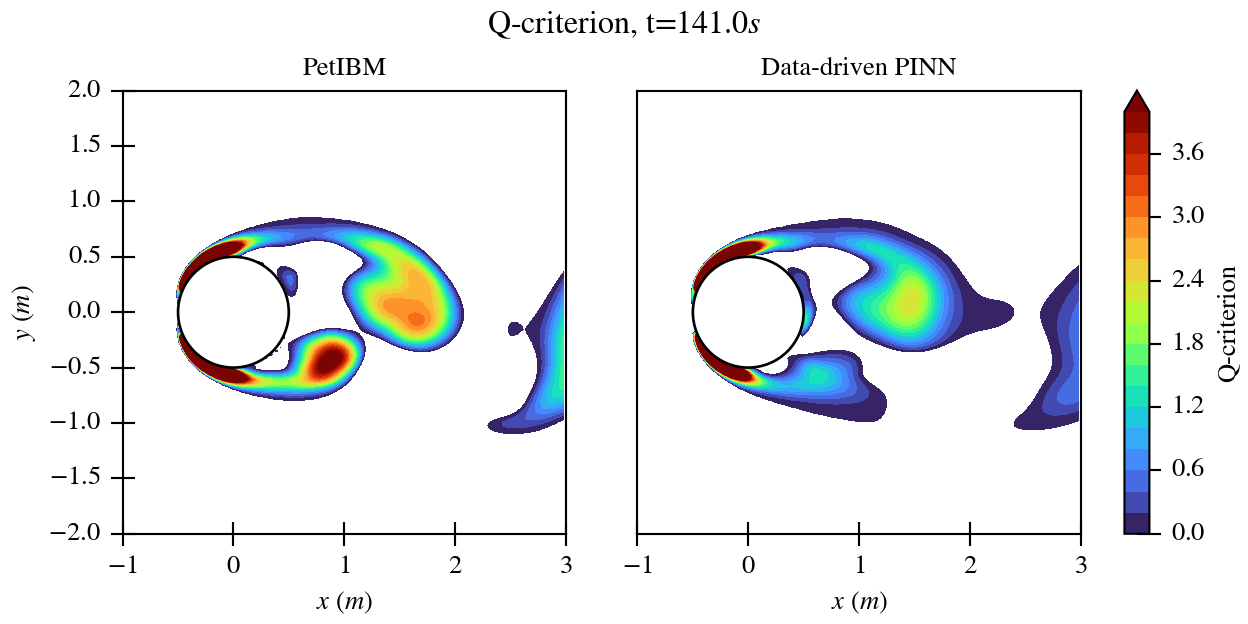
\includegraphics[width=0.95\columnwidth]{cylinder-2d-re200/qcriterion_t141.0.png}%
    \caption{%
        Q-criterion near the cylinder for 2D cylinder flow at $Re=\num{200}$ at $t=141$ w/ data-driven PINNs
    }
    \label{fig:cylinder-re200-pinn-qcrit-t141.0}%
\end{figure}

\begin{figure}[!hbt]
    \centering%
    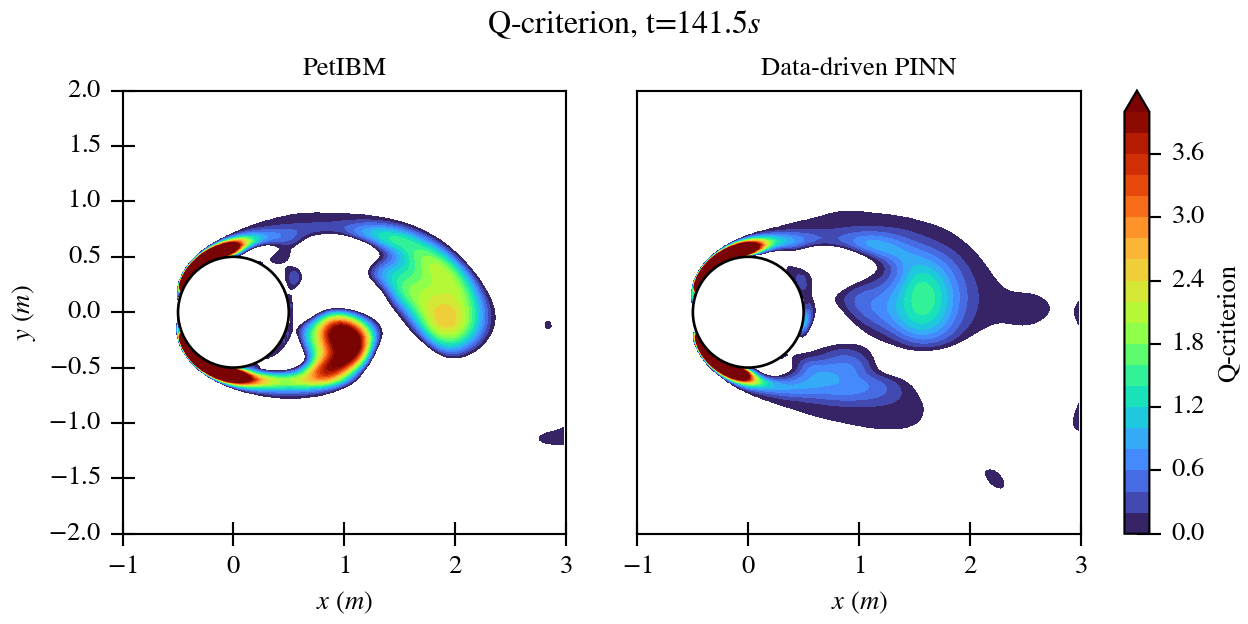
\includegraphics[width=0.95\columnwidth]{cylinder-2d-re200/qcriterion_t141.5.png}%
    \caption{%
        Q-criterion near the cylinder for 2D cylinder flow at $Re=\num{200}$ at $t=141.5$ w/ data-driven PINNs
    }
    \label{fig:cylinder-re200-pinn-qcrit-t141.5}%
\end{figure}

\begin{figure}[!hbt]
    \centering%
    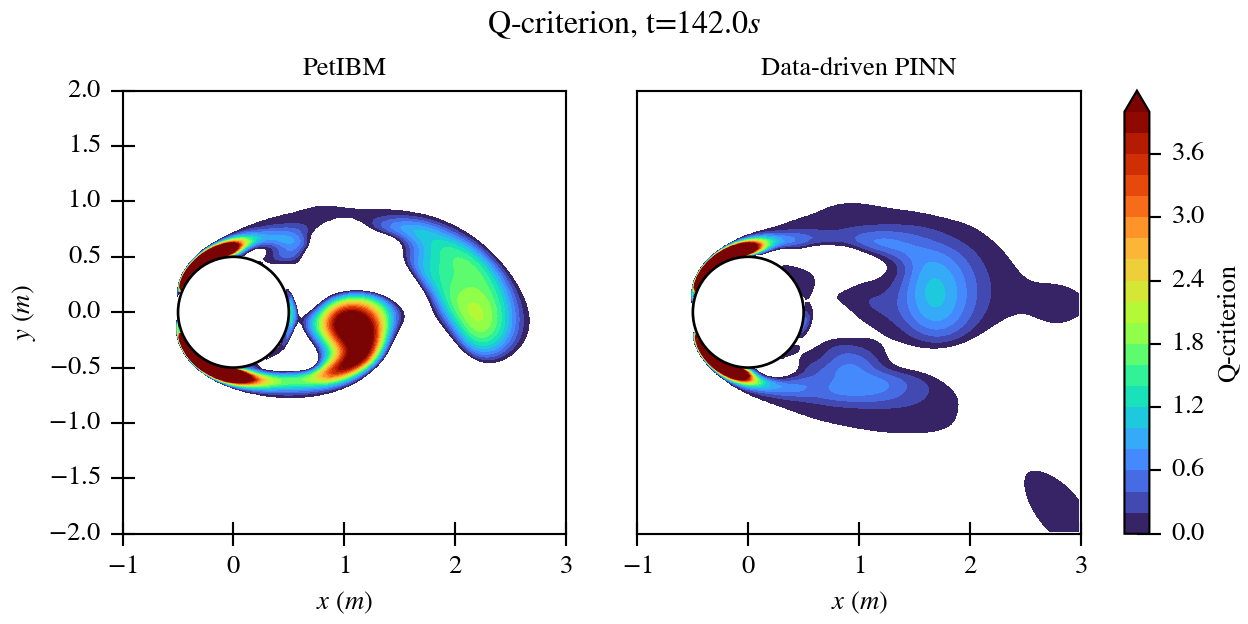
\includegraphics[width=0.95\columnwidth]{cylinder-2d-re200/qcriterion_t142.0.png}%
    \caption{%
        Q-criterion near the cylinder for 2D cylinder flow at $Re=\num{200}$ at $t=142$ w/ data-driven PINNs
    }
    \label{fig:cylinder-re200-pinn-qcrit-t142.0}%
\end{figure}

\begin{figure}[!hbt]
    \centering%
    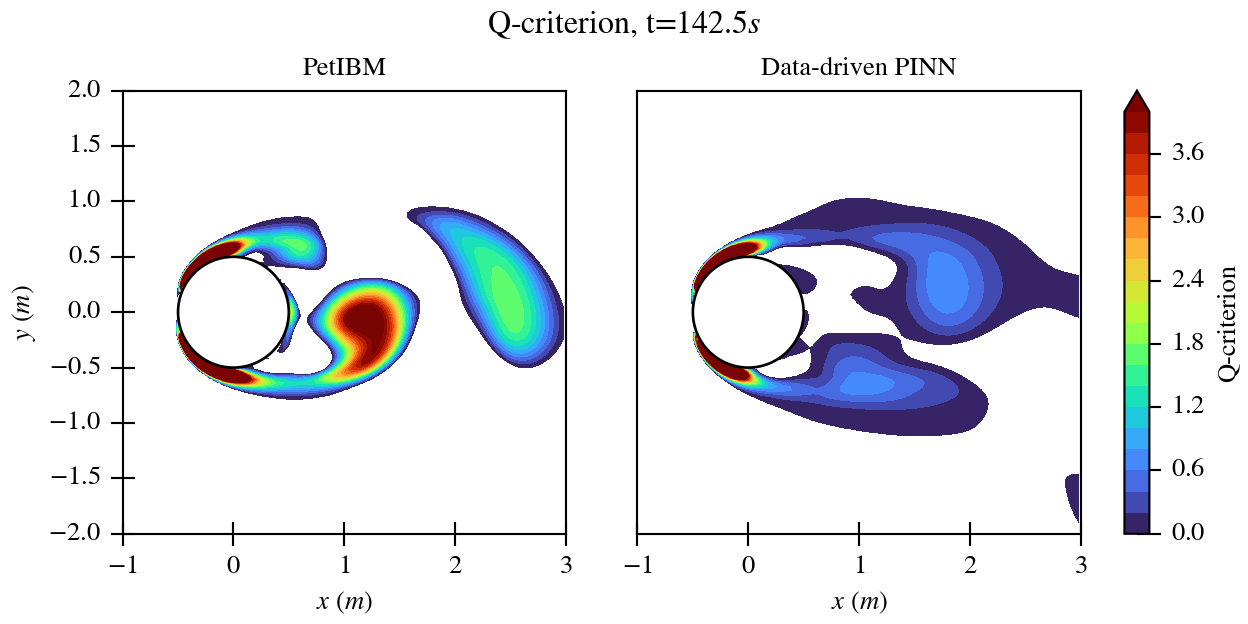
\includegraphics[width=0.95\columnwidth]{cylinder-2d-re200/qcriterion_t142.5.png}%
    \caption{%
        Q-criterion near the cylinder for 2D cylinder flow at $Re=\num{200}$ at $t=142.5$ w/ data-driven PINNs
    }
    \label{fig:cylinder-re200-pinn-qcrit-t142.5}%
\end{figure}

\begin{figure}[!hbt]
    \centering%
    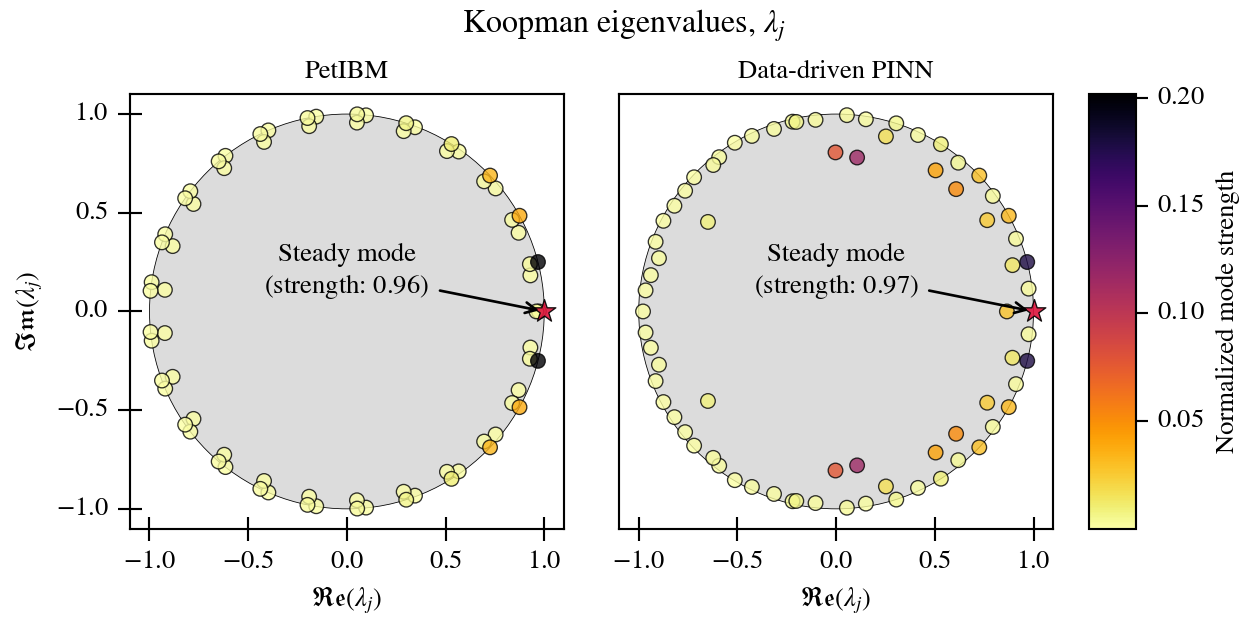
\includegraphics[width=0.95\columnwidth]{cylinder-2d-re200/koopman_eigenvalues_complex}%
    \caption{%
        Distribution of the Koopman eigenvalues on the complex plane for 2D cylinder flow at $Re=\num{200}$.
    }
    \label{fig:cylinder-re200-koopman-eig-dist}%
\end{figure}

\begin{figure}[!hbt]
    \centering%
    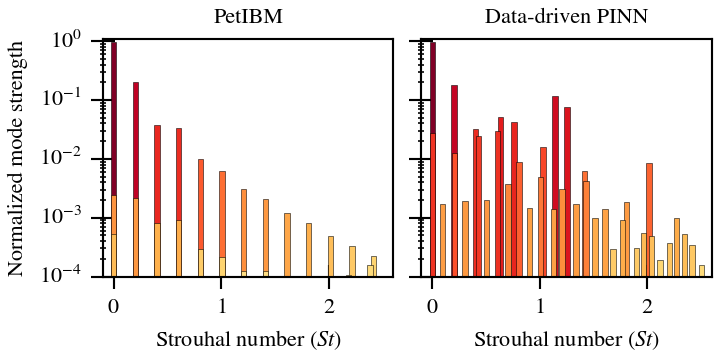
\includegraphics[width=0.95\columnwidth]{cylinder-2d-re200/koopman_mode_strength}%
    \caption{%
        Mode strengths versus mode frequencies for 2D cylinder flow at $Re=\num{200}$.
    }
    \label{fig:cylinder-re200-koopman-mode-strength}%
\end{figure}

\begin{table}[hbt!]
    \begin{threeparttable}[b]
        \begin{tabular}{ccccc}
            \toprule
            $St$ & Strength & Growth Rate & Contours \\
            \midrule
            0     & 0.96 & 1.3e-7  & Figure \ref{fig:cylinder-re200-koopman-petibm-1st}\\
            0.201 & 0.20 & -4.3e-7 & Figure \ref{fig:cylinder-re200-koopman-petibm-2nd}\\
            0.403 & 0.04 & 1.7e-6  & Figure \ref{fig:cylinder-re200-koopman-petibm-3rd}\\
            0.604 & 0.03 & 2.7e-6  & Figure \ref{fig:cylinder-re200-koopman-petibm-4th}\\
            \bottomrule
        \end{tabular}%
        \caption{%
            2D Cylinder, $Re=200$: top 4 primary dynamic modes (sorted by strengths) for PetIBM%
        }%
        \label{table:koopman-petibm}
    \end{threeparttable}
\end{table}%

\begin{table}[hbt!]
    \begin{threeparttable}[b]
        \begin{tabular}{ccccc}
            \toprule
            $St$ & Strength & Growth Rate & Contours \\
            \midrule
            0     & 0.97 & -2.2e-6  & Figure \ref{fig:cylinder-re200-koopman-pinn-primary-1st}\\
            0.201 & 0.18 & -9.4e-6  & Figure \ref{fig:cylinder-re200-koopman-pinn-primary-2nd}\\
            0.403 & 0.03 &  2.3e-5  & Figure \ref{fig:cylinder-re200-koopman-pinn-primary-3rd}\\
            0.604 & 0.03 & -8.6e-5  & Figure \ref{fig:cylinder-re200-koopman-pinn-primary-4th}\\
            \bottomrule
        \end{tabular}%
        \caption{%
            2D Cylinder, $Re=200$: top 4 primary dynamic modes (sorted by strengths) for PINN%
        }%
        \label{table:koopman-pinn-primary}
    \end{threeparttable}
\end{table}%

\begin{table}[hbt!]
    \begin{threeparttable}[b]
        \begin{tabular}{ccccc}
            \toprule
            $St$ & Strength & Growth Rate & Contours \\
            \midrule
            1.142 & 0.12 & -0.24 & Figure \ref{fig:cylinder-re200-koopman-pinn-damped-1st}\\
            1.253 & 0.08 & -0.22 & Figure \ref{fig:cylinder-re200-koopman-pinn-damped-2nd}\\
            0.633 & 0.05 & -0.14 & Figure \ref{fig:cylinder-re200-koopman-pinn-damped-3rd}\\
            0.761 & 0.04 & -0.13 & Figure \ref{fig:cylinder-re200-koopman-pinn-damped-4th}\\
            \bottomrule
        \end{tabular}%
        \caption{%
            2D Cylinder, $Re=200$: top 4 damped dynamic modes (sorted by strengths) for PINN%
        }%
        \label{table:koopman-pinn-damped}
    \end{threeparttable}
\end{table}%

\begin{figure*}[!hbt]
    \centering%
    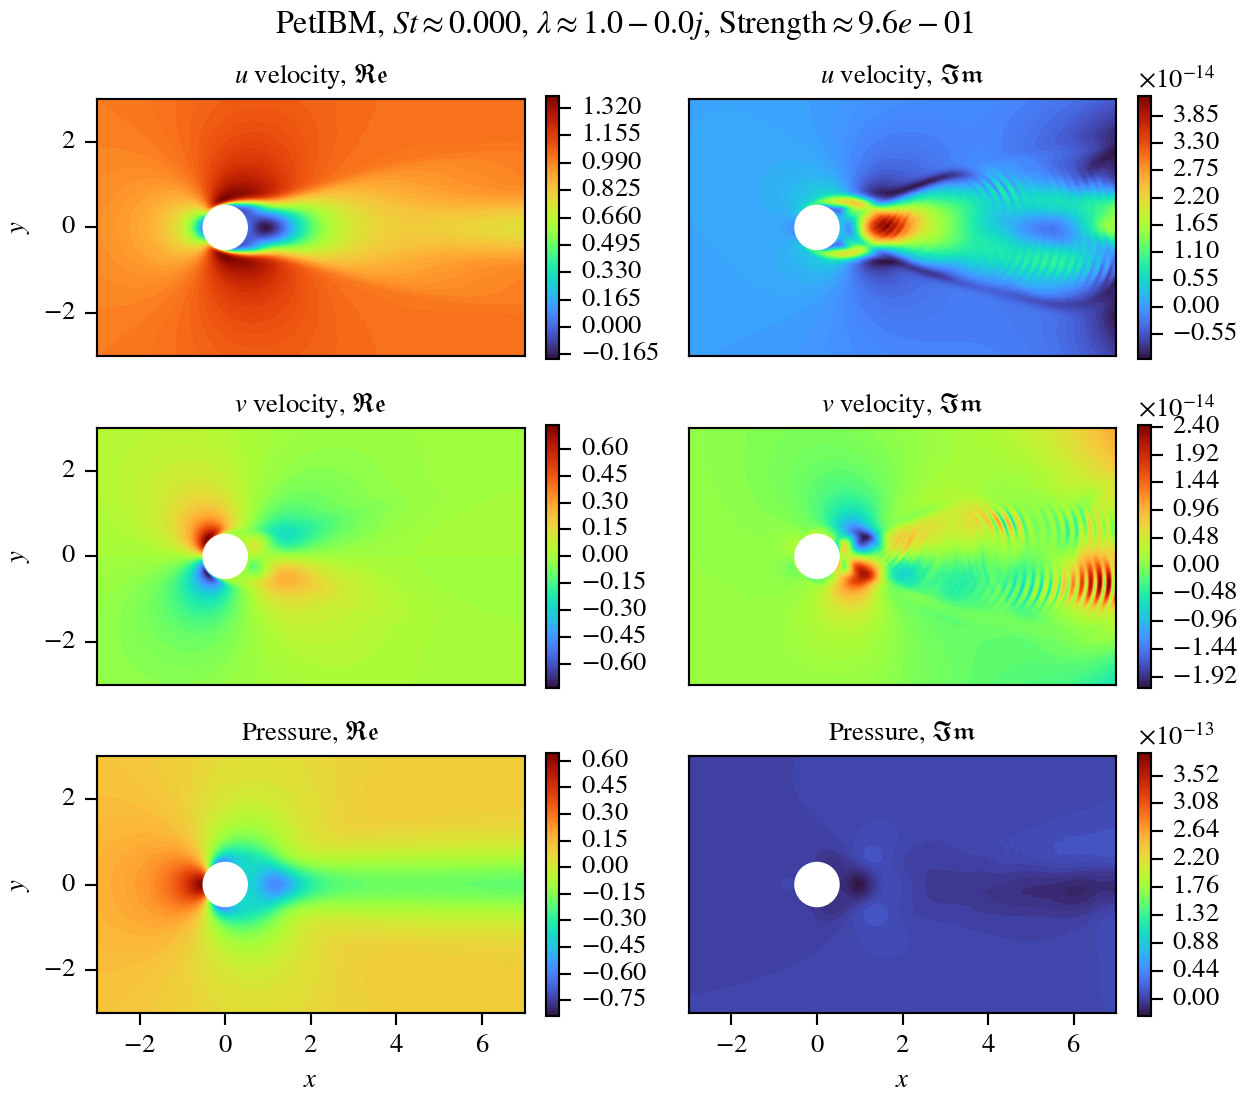
\includegraphics[width=0.8\linewidth]{cylinder-2d-re200/koopman_petibm_000_st0.000.png}%
    \caption{%
        The \num{1}st mode in PetIBM.
    }
    \label{fig:cylinder-re200-koopman-petibm-1st}%
\end{figure*}

\begin{figure*}[!hbt]
    \centering%
    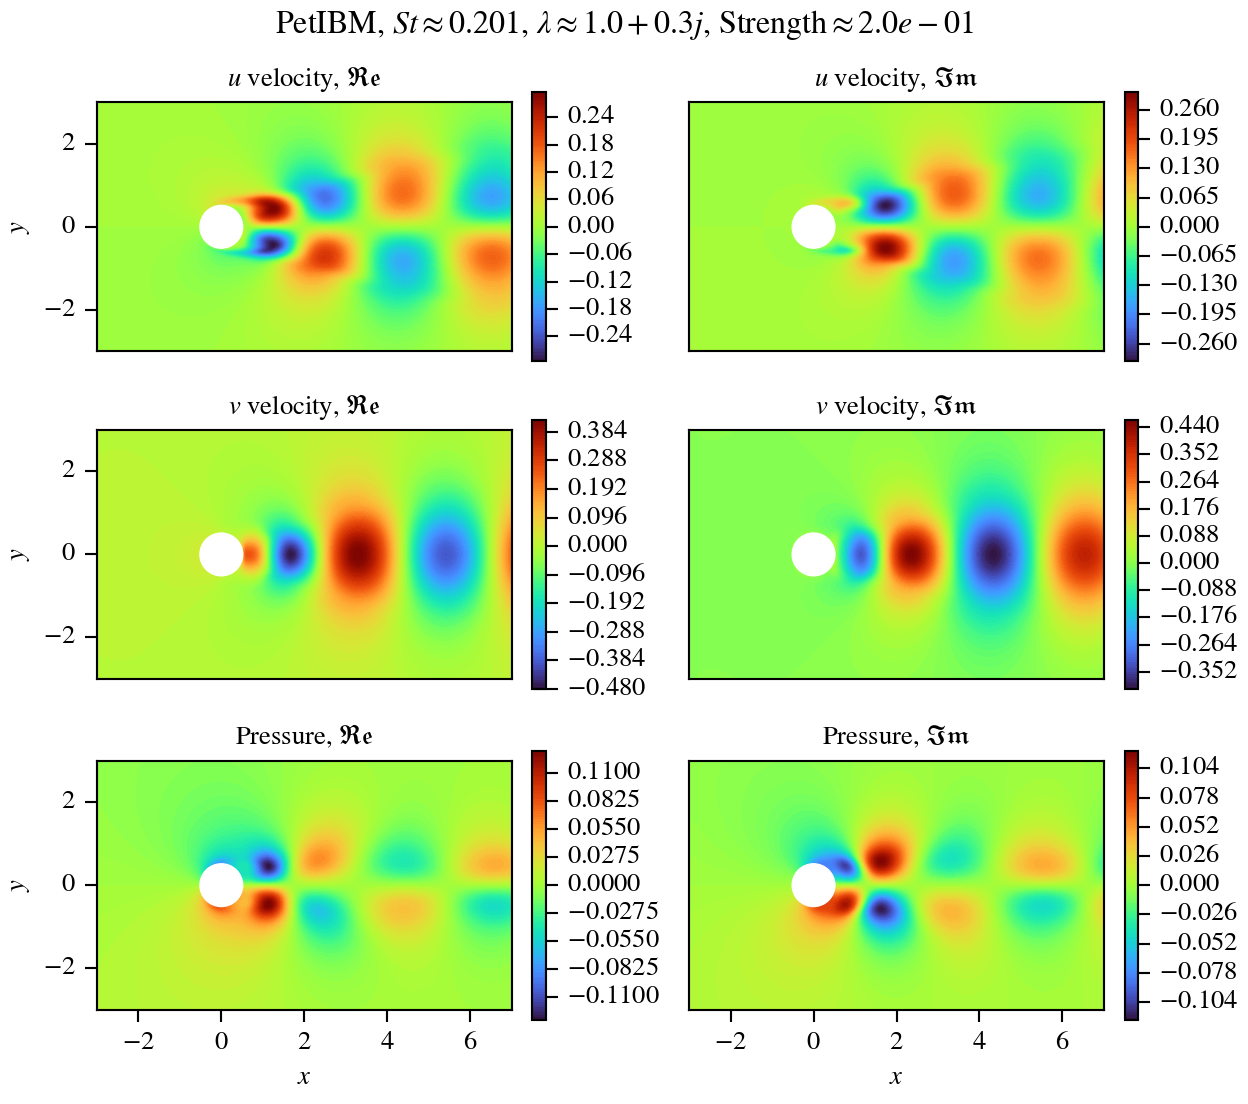
\includegraphics[width=0.8\linewidth]{cylinder-2d-re200/koopman_petibm_001_st0.201.png}%
    \caption{%
        The \num{2}nd mode in PetIBM.
    }
    \label{fig:cylinder-re200-koopman-petibm-2nd}%
\end{figure*}

\begin{figure*}[!hbt]
    \centering%
    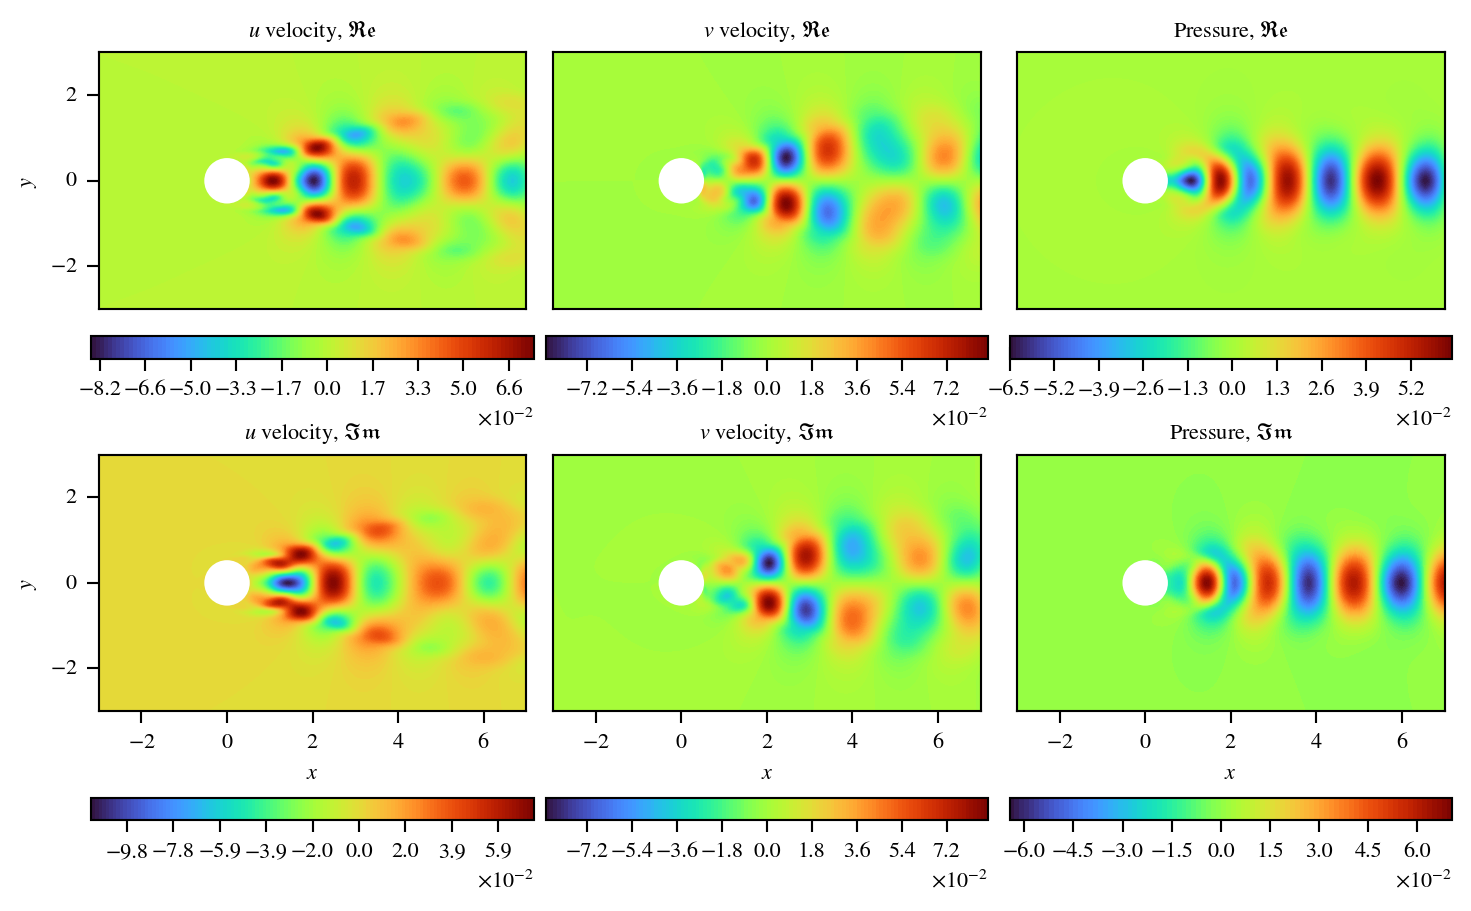
\includegraphics[width=0.8\linewidth]{cylinder-2d-re200/koopman_petibm_002_st0.403.png}%
    \caption{%
        The \num{3}rd mode in PetIBM.
    }
    \label{fig:cylinder-re200-koopman-petibm-3rd}%
\end{figure*}

\begin{figure*}[!hbt]
    \centering%
    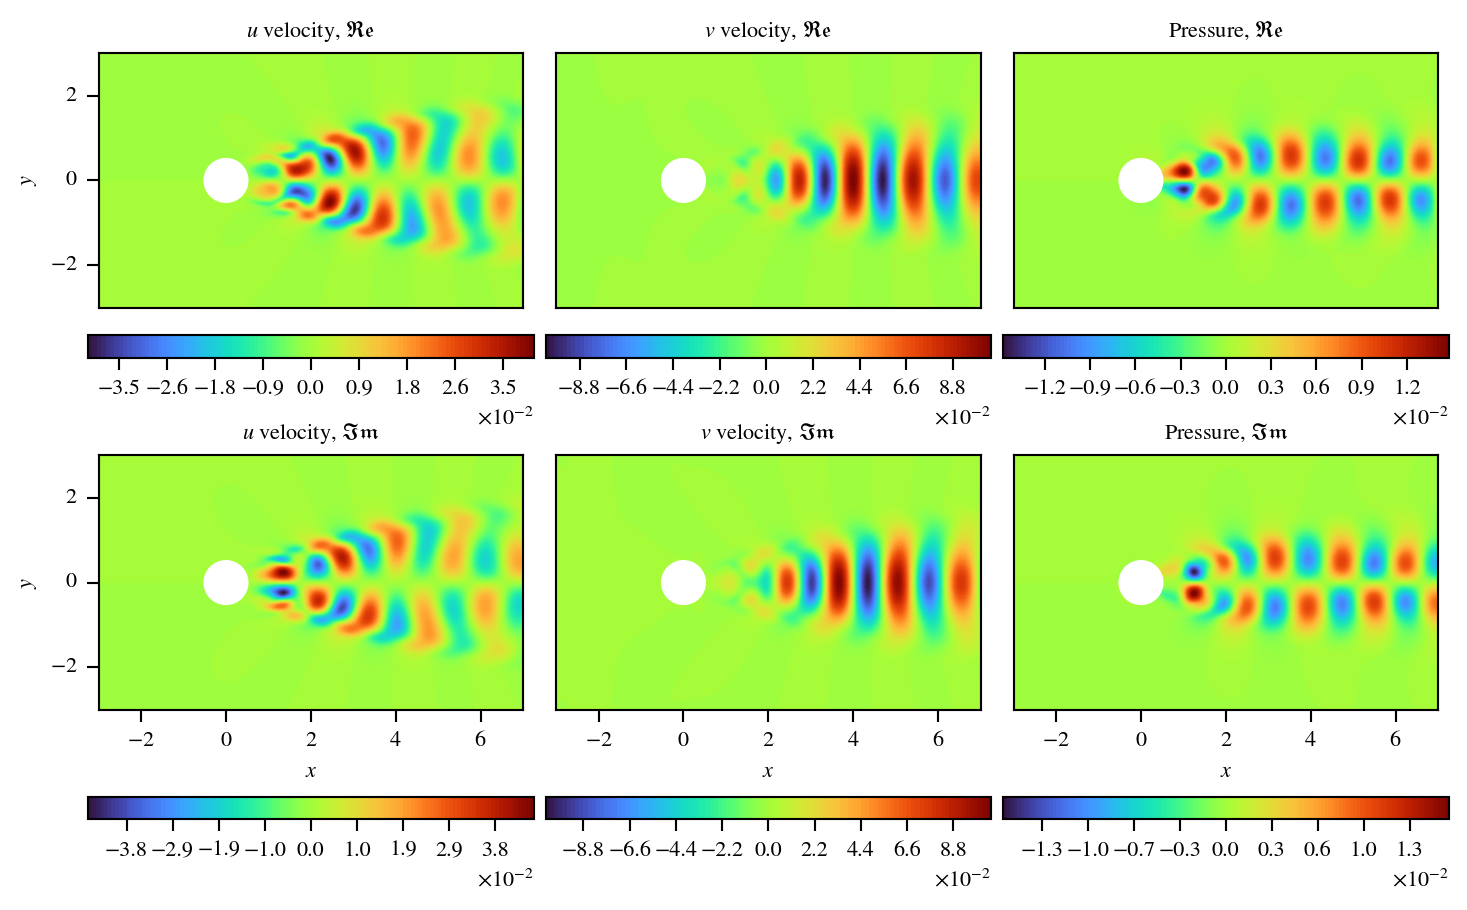
\includegraphics[width=0.8\linewidth]{cylinder-2d-re200/koopman_petibm_003_st0.604.png}%
    \caption{%
        The \num{4}th mode in PetIBM.
    }
    \label{fig:cylinder-re200-koopman-petibm-4th}%
\end{figure*}

\begin{figure*}[!hbt]
    \centering%
    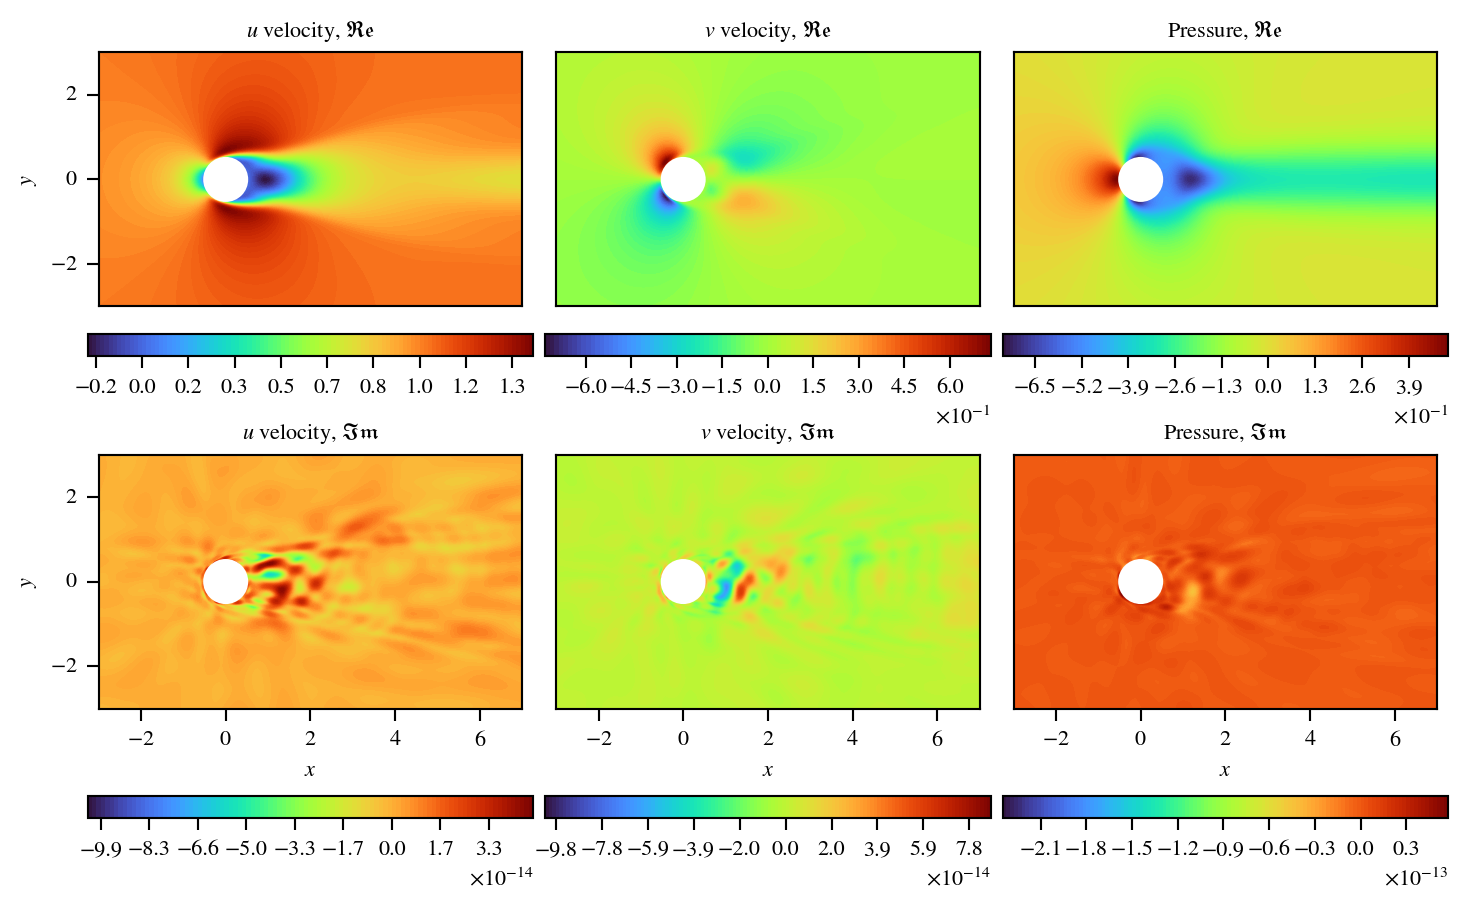
\includegraphics[width=0.8\linewidth]{cylinder-2d-re200/koopman_pinn_000_st0.000.png}%
    \caption{%
        The \num{1}st primary mode in data-driven PINN.
    }
    \label{fig:cylinder-re200-koopman-pinn-primary-1st}%
\end{figure*}

\begin{figure*}[!hbt]
    \centering%
    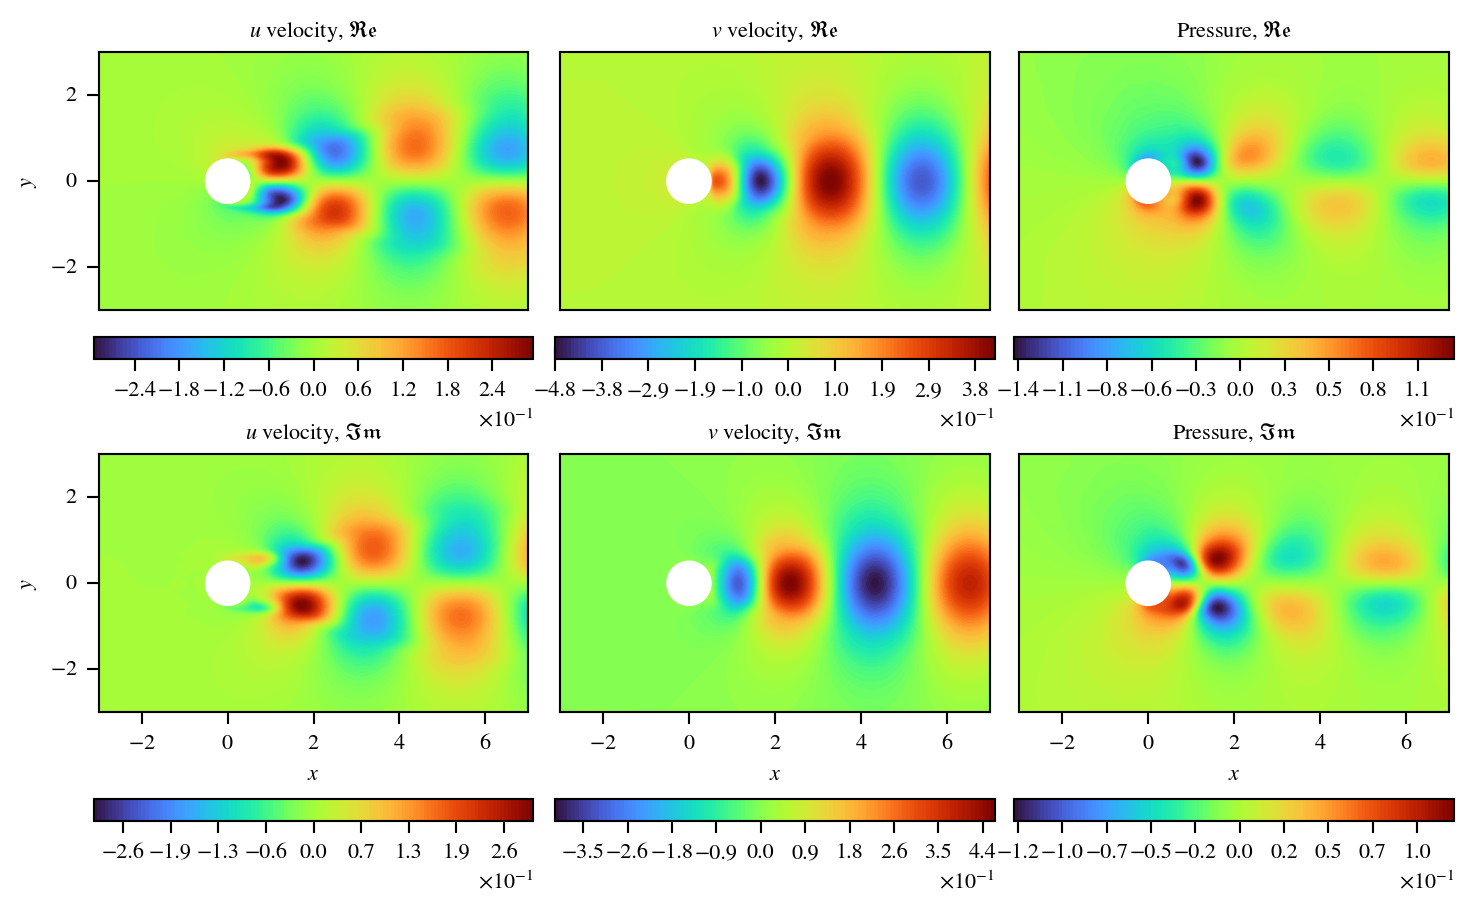
\includegraphics[width=0.8\linewidth]{cylinder-2d-re200/koopman_pinn_001_st0.201.png}%
    \caption{%
        The \num{2}nd primary mode in data-driven PINN.
    }
    \label{fig:cylinder-re200-koopman-pinn-primary-2nd}%
\end{figure*}

\begin{figure*}[!hbt]
    \centering%
    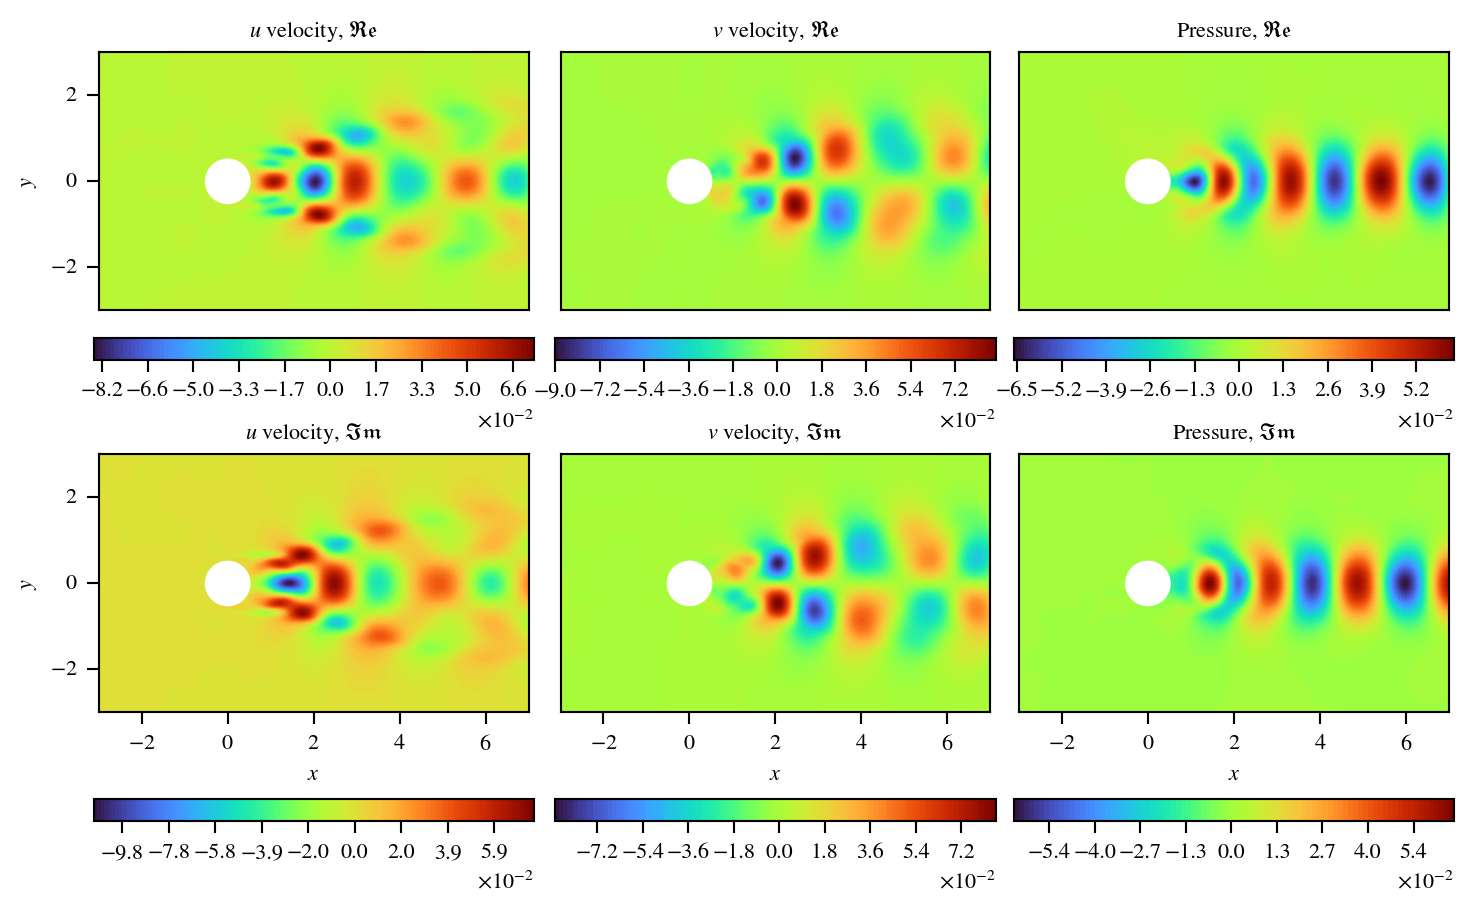
\includegraphics[width=0.8\linewidth]{cylinder-2d-re200/koopman_pinn_006_st0.403.png}%
    \caption{%
        The \num{3}rd primary mode in data-driven PINN.
    }
    \label{fig:cylinder-re200-koopman-pinn-primary-3rd}%
\end{figure*}

\begin{figure*}[!hbt]
    \centering%
    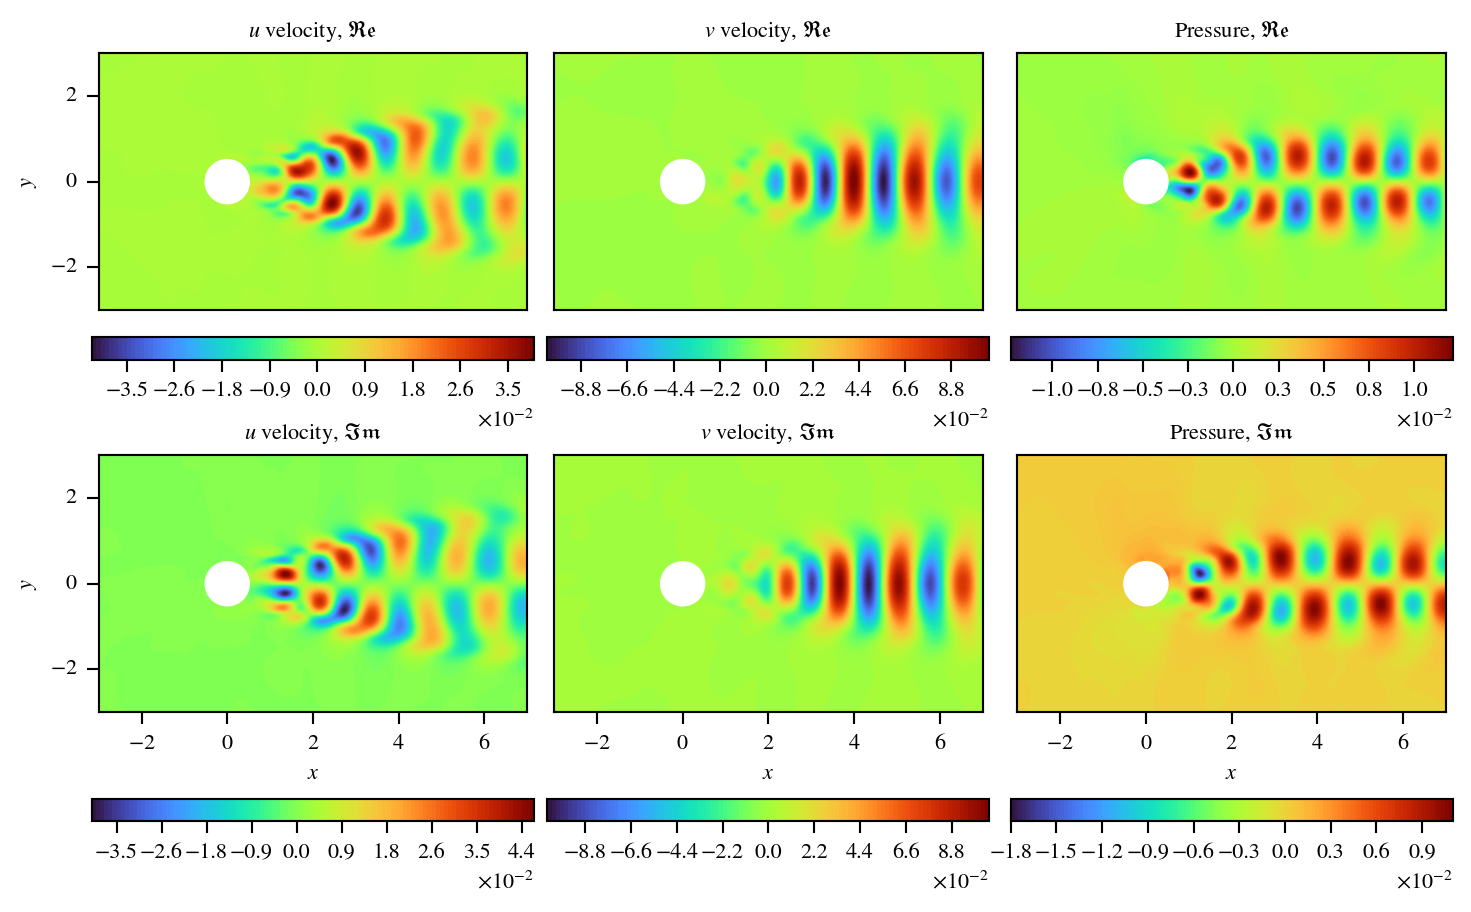
\includegraphics[width=0.8\linewidth]{cylinder-2d-re200/koopman_pinn_007_st0.604.png}%
    \caption{%
        The \num{4}th primary mode in data-driven PINN.
    }
    \label{fig:cylinder-re200-koopman-pinn-primary-4th}%
\end{figure*}

\begin{figure*}[!hbt]
    \centering%
    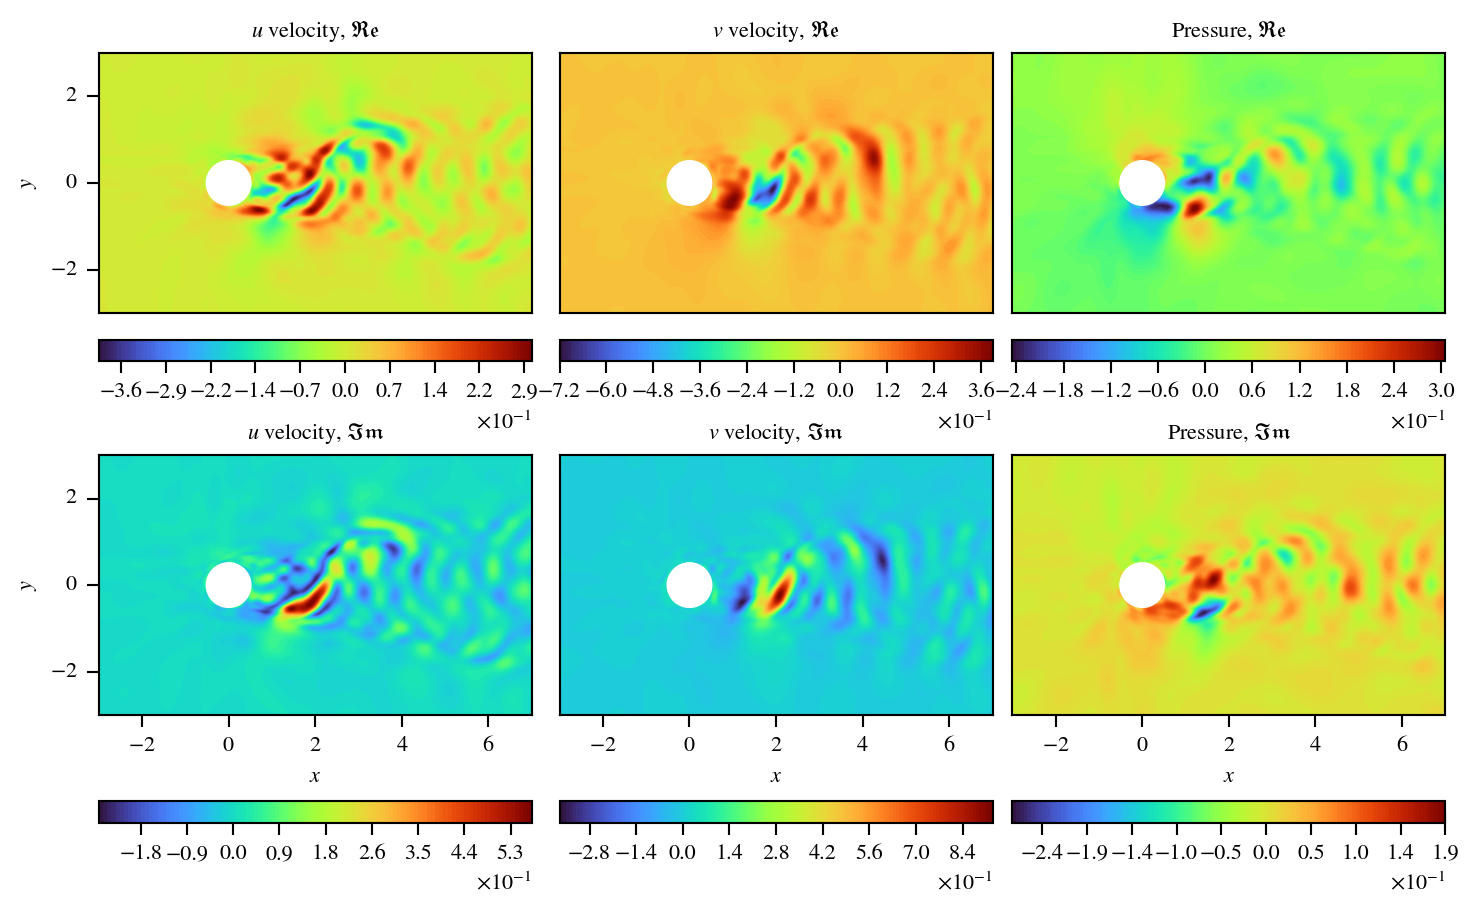
\includegraphics[width=0.8\linewidth]{cylinder-2d-re200/koopman_pinn_002_st1.142.png}%
    \caption{%
        The \num{1}st damped mode in data-driven PINN.
    }
    \label{fig:cylinder-re200-koopman-pinn-damped-1st}%
\end{figure*}

\begin{figure*}[!hbt]
    \centering%
    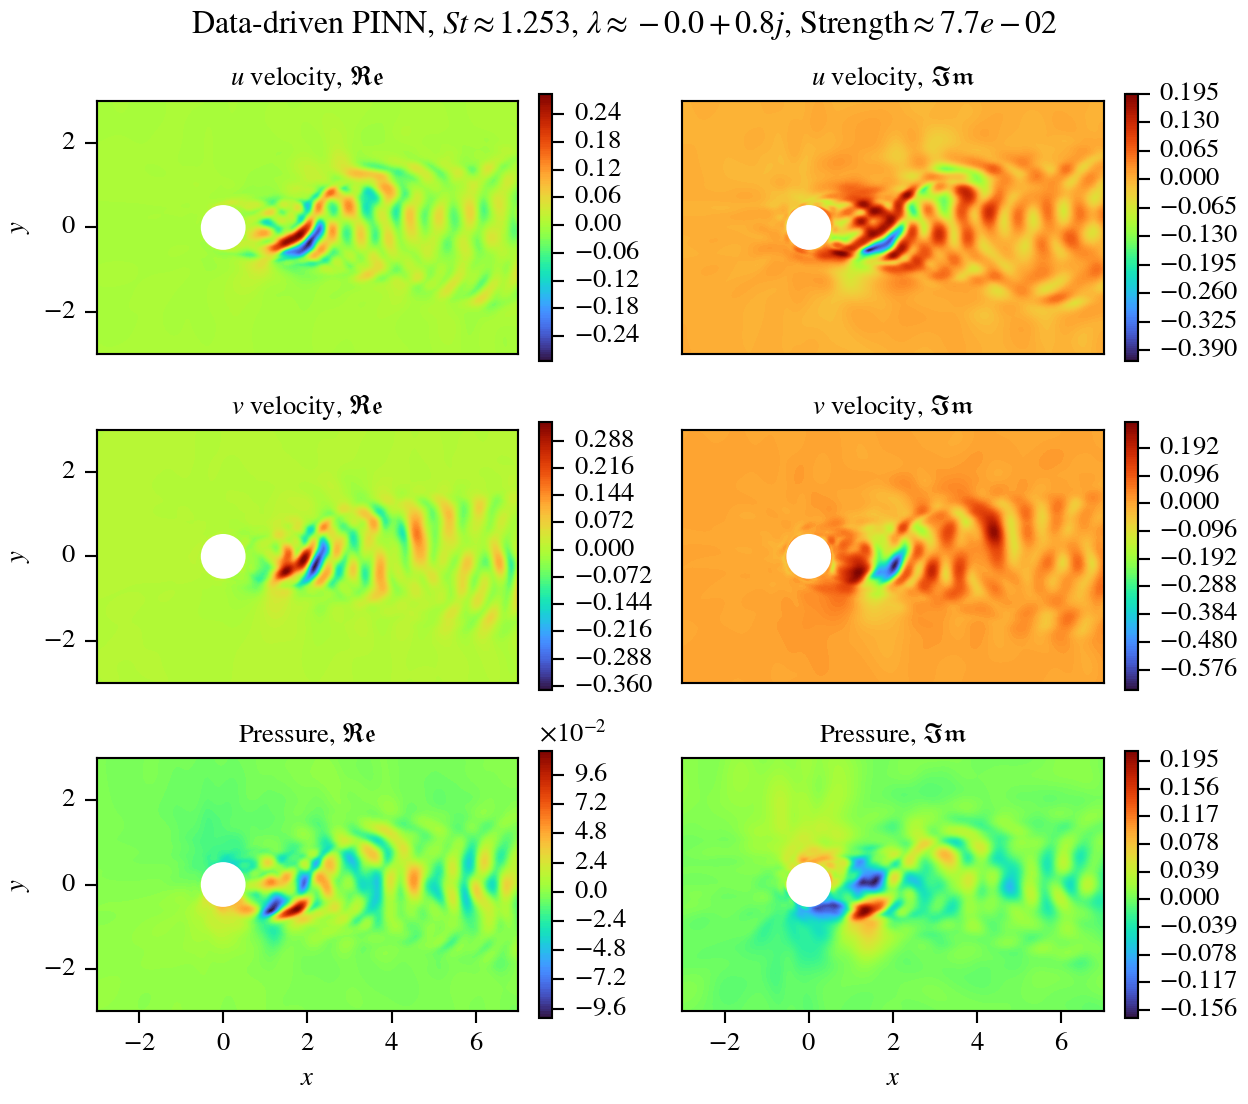
\includegraphics[width=0.8\linewidth]{cylinder-2d-re200/koopman_pinn_003_st1.253.png}%
    \caption{%
        The \num{2}nd damped mode in data-driven PINN.
    }
    \label{fig:cylinder-re200-koopman-pinn-damped-2nd}%
\end{figure*}

\begin{figure*}[!hbt]
    \centering%
    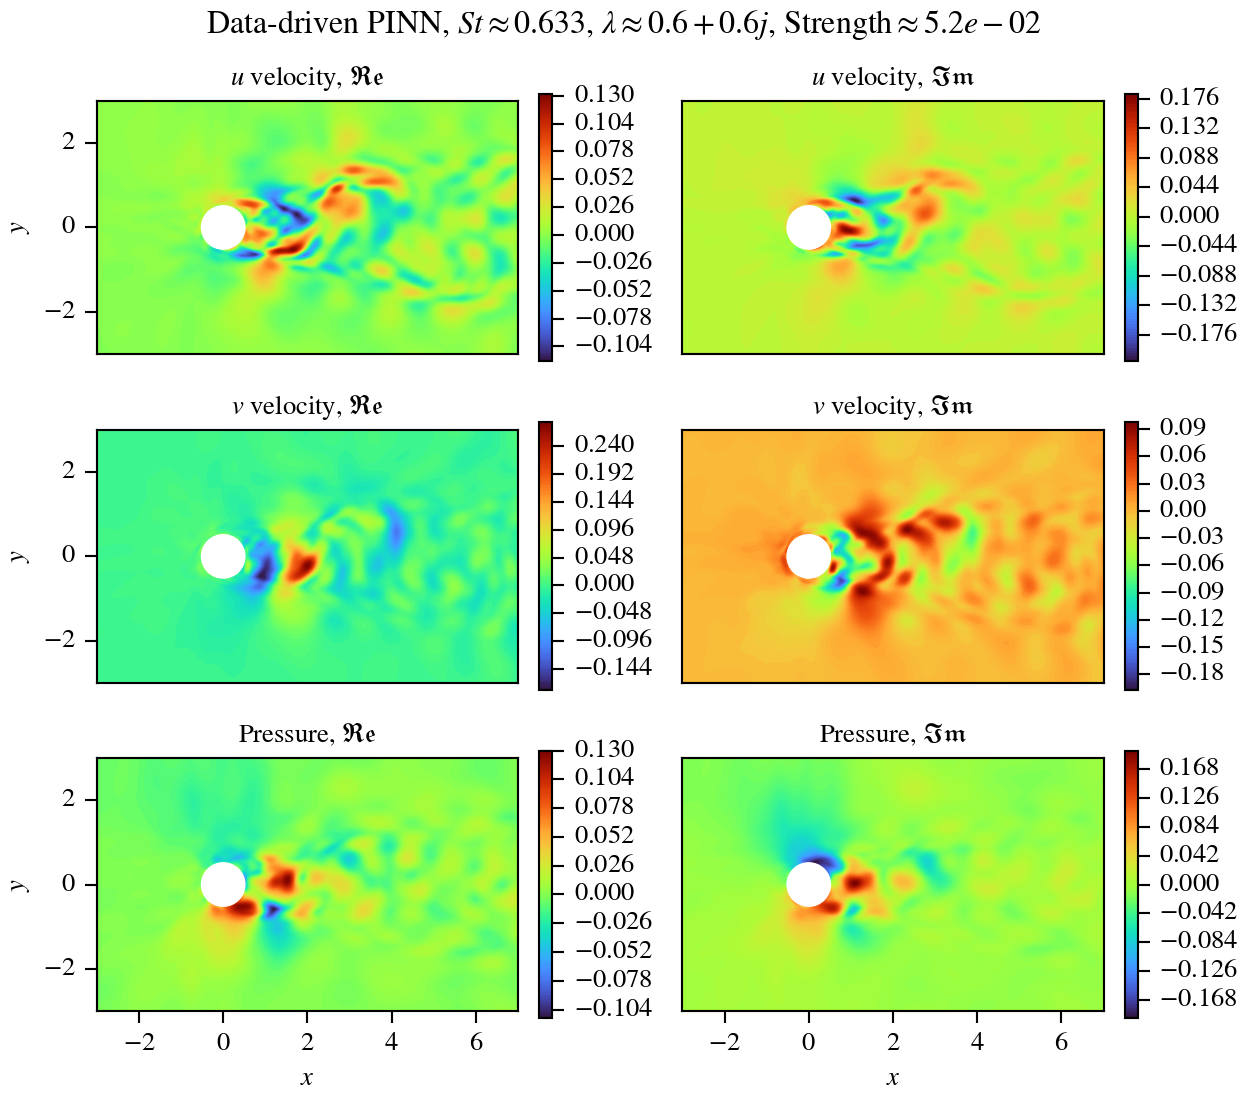
\includegraphics[width=0.8\linewidth]{cylinder-2d-re200/koopman_pinn_004_st0.633.png}%
    \caption{%
        The \num{3}rd damped mode in data-driven PINN.
    }
    \label{fig:cylinder-re200-koopman-pinn-damped-3rd}%
\end{figure*}

\begin{figure*}[!hbt]
    \centering%
    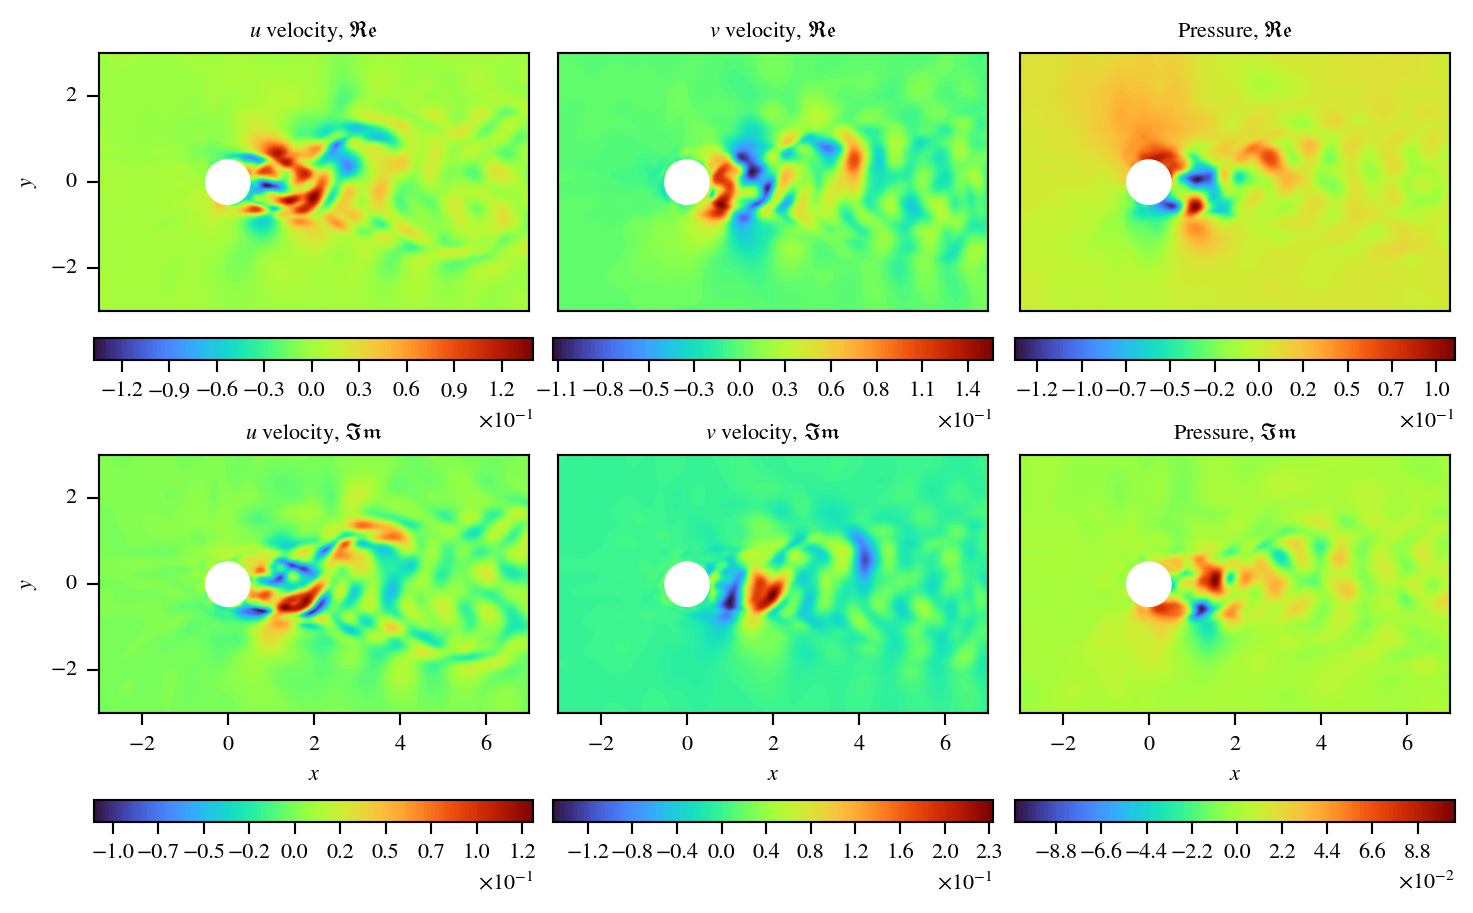
\includegraphics[width=0.8\linewidth]{cylinder-2d-re200/koopman_pinn_005_st0.761.png}%
    \caption{%
        The \num{4}th damped mode in data-driven PINN.
    }
    \label{fig:cylinder-re200-koopman-pinn-damped-4th}%
\end{figure*}

% vim:ft=tex:
